\documentclass{uhcoethesis}

\title{Design, Modeling and Control of the Intelligent Bio-Inspired Underwater Robotics for Safety Inspection}
\author{Muhammad Umar Masood}
\department{Department of Mechanical and Aerospace Engineering}
\degree{Doctor of Philosophy}
\major{Mechanical Engineering}
\degreedate{August 2026}
\submissiontype{dissertation}
\chair{Zheng Chen}
\committeemember{Gangbing Song}
\committeemember{Karolos Grigoriadis}
\committeemember{Marzia Cescon}
\committeemember{Aaron T. Becker}

\begin{document}

\frontmatter
\maketitlepage
% Uncomment if you need the optional copyright page.
\makecopyrightpage

\begin{dedication}
I dedicate this work to my mother who visioned me having a Ph.D. when I was a child and to my late father who always supported and groomed me to what I am today.
\end{dedication}

\begin{acknowledgements}
I acknowledge the support and guidance of my advisor, Dr. Zheng Chen, for his mentorship and encouragement throughout my Ph.D. journey. I am grateful to my committee members, Dr. Gangbing Song, Dr. Karolos Grigoriadis, Dr. Marzia Cescon, and Dr. Aaron T. Becker, for their valuable feedback and insights that have significantly contributed to the quality of this dissertation.\\
Special thanks to my wife, Uzma, for her unwavering support and understanding during the challenging times of my research, and to my son, Abdullah, for being a source of joy and inspiration. Finally, I am grateful to my family for their love and encouragement, which has been instrumental in my academic journey. I would also thank my brothers, Naeem and Mohsin, and my sister Khadija for always encouraging me during the ups and downs of my Ph.D. journey. At this moment, I can't forget my professional colleagues at Bio-inspired Robotics and Control Lab (BRCL), Qiang Zhu, Alejandro Salvador, Denizcan Koc, and Dr. Theopilus Kaaya, for their support and collaboration in my research work.\\
I owe my deepest gratitude to the University of Houston for providing me with the resources and opportunities to pursue my research and academic goals, and the financial support from Subsea Systems Institute (SSI) at UH Energy, National Science Foundation (NSF), Bureau of Safety and Environmental Enforcement (BSEE), Center for Carbon Management and Energy (CCME), and Offshore Energy Safety Institute (OESI) for funding my research work.
\end{acknowledgements}

\begin{abstractpage}
The transition toward low-carbon energy systems requires reliable monitoring of underwater infrastructure, including subsea pipelines, carbon dioxide sequestration sites, and environmentally sensitive marine environments. Conventional underwater vehicles are often limited by high cost, limited maneuverability in confined regions, and dependence on bulky sensing and localization systems. This dissertation presents the design, modeling, and control of an intelligent bio-inspired robotic fish platform for energy-transition applications, with emphasis on pipeline tracking, environmental sensing, depth regulation, and underwater relative localization.

The robotic fish is developed as a compact, low-cost, and maneuverable underwater platform integrating bio-inspired propulsion, embedded sensing, vision-based perception, depth-control hardware, and wireless sensing modules. A system-level design framework is presented, including mechanical design, electronics integration, actuator selection, buoyancy management, and real-time embedded control. Dynamic models are developed for key subsystems, including the robotic fish motion and a variable-buoyancy/depth-control device. Model-based and feedback control strategies are implemented to regulate swimming behavior and depth while accounting for actuator constraints and practical experimental limitations.

For infrastructure monitoring, the dissertation develops vision-based pipeline tracking methods that allow the robotic fish to detect and follow underwater pipeline-like features using onboard camera feedback. Environmental monitoring capabilities are investigated through oil-spill sensing experiments and carbon dioxide leak-source localization concepts relevant to subsea sequestration monitoring. In addition, an underwater relative-localization framework is developed using received signal strength indicator measurements from multiple antenna channels, fused with inertial and magnetic sensing to estimate relative distance and bearing between underwater nodes or robotic platforms.

The proposed methods are validated through hardware development, benchtop testing, pool experiments, and data-driven analysis. The results demonstrate that an intelligent robotic fish can serve as an integrated experimental platform for underwater mobility, sensing, and autonomy in energy-transition applications. By combining bio-inspired locomotion, depth control, visual servoing, environmental sensing, and RSS-based localization, this work contributes toward scalable autonomous underwater systems for safer monitoring of subsea infrastructure and emerging carbon-management technologies.
\end{abstractpage}

\tableofcontents
\newpage
\listoftables
\newpage
\listoffigures

\mainmatter

\chapter{Introduction}

Oceans cover more than 70\% of the Earth's surface and support climate regulation, transportation, energy production, communication infrastructure, and marine ecosystems \cite{ocean_ngs,noaa_ocean_exploration}. They also host an expanding network of engineered assets, including subsea pipelines, offshore energy facilities, communication cables, and carbon-management infrastructure. These assets are difficult to observe directly because underwater environments impose limited visibility, high pressure, uncertain currents, strong attenuation of electromagnetic signals, and substantial operational cost for deployment and recovery. As a result, inspection and monitoring remain central problems in ocean engineering, offshore safety, and environmental protection \cite{Ho2020,Shukla2016,Mcleod2012,Patel2024}.

The monitoring problem is becoming broader rather than narrower. Traditional offshore oil and gas infrastructure still requires inspection for corrosion, mechanical damage, leakage, and environmental contamination. At the same time, carbon capture and storage (CCS) technologies are creating new subsea monitoring needs because captured \mbox{CO$_2$} must be transported and stored without uncontrolled release \cite{Herzog2001,Yadav2022,Osman2021}. Failures in these systems can release hydrocarbons or \mbox{CO$_2$} into aquatic environments, with consequences that include ecological toxicity, seawater acidification, and long-term disturbance to marine habitats \cite{Filonchyk2024,Kabir2023,Zheng2021,Mortezaei2021,queiros2014potential,Pham2016}. Reliable monitoring therefore requires not only leak detection, but also spatial inspection, mobile sensing, and the ability to collect measurements near the region of interest.

Conventional underwater monitoring is often built around large remotely operated vehicles (ROVs), autonomous underwater vehicles (AUVs), fixed instrumentation, or surface-vessel operations. These approaches are necessary for many industrial tasks, but they are not always suitable for low-cost, repeated, or low-disturbance inspection. They can require high-cost vessels, trained crews, heavy tethers, large acoustic systems, or significant mission-planning overhead \cite{Capocci2017,Shukla2016,Mcleod2012}. For sensitive environments, the propulsion and operational footprint of conventional systems can also disturb sediment or biological activity near the inspection site \cite{Marras2012,Polverino2013}. This motivates research into compact underwater robots that can operate as mobile sensing platforms with lower cost and lower environmental disturbance.

This dissertation addresses this need through the development and use of a compact bio-inspired robotic fish platform. The thesis does not treat robotic-fish locomotion, buoyancy control, perception, chemical sensing, and localization as isolated topics. Instead, these topics are developed as connected capabilities required for a small underwater robot to inspect infrastructure, collect environmental measurements, regulate its position in three-dimensional water environments, and move toward cooperative monitoring. The introduction establishes the motivation and prior work across the four main technical directions of the dissertation: design and modeling of the underwater robot and buoyancy device, model validation and control design, safety inspection and monitoring of underwater infrastructure, and cooperative inspection through relative localization. Detailed hardware drawings, equations, controller synthesis, sensing algorithms, and experimental results are reserved for the corresponding technical chapters.

\section{Underwater Infrastructure Monitoring}

Subsea infrastructure monitoring has long been a central activity in offshore oil and gas operations, where pipelines must be inspected for corrosion, impact damage, leakage, biofouling, and structural degradation \cite{Ho2020,Shukla2016}. The pipeline network is exposed to external loads, pressure cycling, seabed movement, corrosion, material defects, and accidental impact. For petroleum infrastructure, leakage can release crude oil or gas into the surrounding environment. For carbon-management infrastructure, leakage can release dense-phase or gaseous \mbox{CO$_2$} into seawater. Although the physical mechanisms differ, both cases require early detection, spatial localization, and follow-up inspection near the suspected leak region.

Pipeline leak detection is commonly divided into internal and external approaches. Internal approaches infer leakage from measurements inside the pipeline, including mass-volume balance, acoustic or pressure-wave methods, pressure point analysis, inverse transient analysis, and simplified pressure-analysis techniques \cite{martins2010assessment,hou2013pipeline,bin2011pressure,vitkovsky2007experimental,ostapkowicz2016leak}. These methods can support continuous surveillance and can often identify that an abnormal condition has occurred. However, they do not directly map the surrounding environment, measure contaminant spread, or inspect the external condition of the pipeline after a suspected event. They are also sensitive to instrumentation quality, flow conditions, and measurement noise, which can increase false alarms or uncertainty in leak localization \cite{reda2024roadmap}.

External approaches inspect the pipeline or the surrounding water directly. These include visual inspection, acoustic monitoring, fiber-optic sensing, fluorometric detection, capacitive sensing, chemical sensing, and robotic surveys \cite{Ho2020,jasper2012oil,lukonge2020leak,adegboye2019recent}. External approaches can provide more direct physical evidence of leakage or contamination, but their value depends on the platform that carries the sensor. Fixed sensors are useful only near their installation point. Surface and aerial systems can observe large-scale surface slicks but are less suitable for early detection near a submerged source. ROV- or AUV-mounted sensors can reach the subsea region, but deployment cost and operational complexity limit how frequently they can be used for small-scale or distributed monitoring.

CCS monitoring adds distinct engineering and environmental constraints. \mbox{CO$_2$} pipelines may experience fracture and decompression behavior influenced by pressure, phase transition, and impurities in the transported stream \cite{Aursand2016,CoshamAtkinsBoreas2009}. If \mbox{CO$_2$} escapes into seawater, it can dissolve and form carbonic acid, locally changing pH and potentially affecting benthic organisms, fish larvae, and other marine communities \cite{Zheng2021,Mortezaei2021,queiros2014potential,Pham2016}. Monitoring therefore must not be limited to the mechanical condition of a pipe. It must also include environmental measurements that can indicate where the leaked substance has moved after release.

Prior work has investigated mobile robotic platforms for related inspection problems. Zhang et al.~\cite{Zhang2021} studied AUV-based subsea pipeline leak inspection. Qasem et al.~\cite{Qasem2019} developed a multisensor ROV for oil-spill surveillance. Hu et al.~\cite{Hu2022} investigated robotic-fish-based underwater gas leak detection using onboard camera data. These studies show that mobile underwater sensing can provide information that fixed instrumentation alone cannot. They also motivate the central systems question of this dissertation: how can a compact bio-inspired robotic fish be designed, controlled, and instrumented so that inspection, environmental sensing, and relative localization can be studied on a common platform?

\section{Limitations of Conventional Platforms}

ROVs and AUVs remain the dominant platforms for subsea inspection. ROVs can carry large payloads and provide real-time operator feedback, but they are tethered systems that require surface vessels, skilled operators, and substantial deployment cost \cite{Capocci2017,Shukla2016}. AUVs reduce tether dependence and can execute preplanned missions, but many are still large, expensive vehicles designed for broad survey tasks rather than compact inspection near confined pipeline corridors or environmentally sensitive regions \cite{Mcleod2012,Patel2024}. In high-value industrial inspection, these costs can be justified because the infrastructure being inspected is expensive and failure can be catastrophic. For repeated environmental monitoring, laboratory-scale method development, distributed coverage, or operation in smaller water bodies, the same cost and logistical requirements become limiting.

The propulsion and sensing footprint of conventional vehicles is another limitation. Many inspection-class vehicles rely on propellers or thrusters to generate maneuvering forces. These devices are effective and controllable, but they can introduce local turbulence, disturb sediment, alter the local sensing environment, and affect marine life in ways that are undesirable for ecological monitoring \cite{Marras2012,Polverino2013}. For chemical sensing, this disturbance can also change the local concentration field by mixing the water near the sensor. For visual inspection, sediment disturbance can reduce visibility and degrade image-based feature extraction. These issues motivate low-speed, low-disturbance vehicle designs when the monitoring task does not require high-speed transit or heavy payload transport.

Navigation and localization impose additional constraints. Global positioning system (GPS) signals do not penetrate seawater, so underwater vehicles commonly rely on acoustic long-baseline (LBL), short-baseline (SBL), or ultra-short-baseline (USBL) systems, sometimes combined with Doppler velocity logs (DVLs) and inertial sensors \cite{Luo2021Review,Su2020,zekavat2019handbook}. These systems can provide high accuracy, but the supporting acoustic hardware, deployment infrastructure, power consumption, and cost are difficult to scale down to small robotic fish or multi-robot groups. Recent acoustic work has sought more compact solutions, including passive inverted ultra-short baseline (piUSBL), passive iUSBL for small AUVs, and MEMS-microphone-based acoustic localization and communication \cite{Rypkema2019piUSBL,Wang2022PassiveIUSBL,Hinduja2022MEMSAcoustic}. These efforts are important, but they do not remove the need for complementary low-cost relative-localization methods that can support compact cooperative monitoring platforms.

The same issue appears in sensing. High-end sonars, Doppler instruments, acoustic positioning systems, and large chemical payloads can be appropriate for full-scale AUVs, but they are not always compatible with small robotic fish. Compact robots require sensors that are lightweight, low-power, waterproof, and compatible with limited onboard processing and communication. The design problem is therefore not only to select a robot body or a sensor independently. The platform, power system, actuator configuration, sensor interfaces, waterproofing, communication pathway, and software must be treated together. This system-level requirement is one of the motivations for developing AquaNavigator as a common experimental platform rather than using unrelated hardware for each monitoring task.

\section{Bio-Inspired Robotic Fish}

Bio-inspired robotic fish offer an alternative class of underwater platform for low-speed, low-disturbance monitoring. Fish-like propulsion is grounded in classical models of aquatic animal locomotion, including Lighthill's elongated-body and large-amplitude elongated-body theories \cite{lighthill1969hydromechanics,Lighthill1971}. Robotic-fish research has since expanded into design, fabrication, hydrodynamics, control, and sensing, with survey work summarizing the state of biomimetic fish robots and body and/or caudal fin swimming mechanisms \cite{Yu2017,Duraisamy2019DesignReview,Xie2021DesignsReview}. Because robotic fish can be compact and can move with oscillatory body or tail motion, they are attractive as mobile sensor platforms for aquatic environments \cite{Tan2011}. Their wake and motion can also be less disruptive to aquatic organisms than rigid propeller-driven platforms in some settings \cite{Marras2012,Polverino2013}.

Prior robotic-fish platforms have demonstrated vision-based target following, visual-inertial localization, soft robotic swimming near coral reefs, and increasingly sophisticated bio-inspired propulsion and motion planning \cite{Hu2009,Wang2015,Katzschmann2018,Li2024,Jiang2024}. Other work has studied dynamic modeling of tail-actuated robotic fish and the relationship between caudal-fin kinematics, thrust, drag, and body motion \cite{Wang2013,Park2012}. Zuo et al.~\cite{Zuo2021} developed a double-slider-crank mechanism for carangiform robotic-fish propulsion, providing a compact mechanical basis for efficient tail-driven swimming. Taken together, these studies establish robotic fish as a credible class of underwater robot for compact locomotion and sensing.

However, the literature also shows a gap between robotic-fish locomotion research and complete monitoring systems. Many robotic fish are developed to demonstrate swimming performance, maneuverability, locomotion efficiency, or tracking of visual targets. Fewer studies integrate the full chain required for underwater monitoring: a physical platform, three-dimensional positioning capability, onboard perception, environmental sensing payloads, and a path toward cooperative operation. For subsea infrastructure monitoring, the robot must not only swim. It must move in a controlled way near a feature, carry sensors without destabilizing the vehicle, regulate its vertical position, collect meaningful measurements, and communicate or localize relative to other agents.

The AquaNavigator platform used in this dissertation is developed within this broader need. It uses bio-inspired tail-driven propulsion as the mobility foundation, but the platform is treated as more than a locomotion prototype. It is the common experimental base through which buoyancy control, pipeline tracking, \mbox{CO$_2$} sensing, oil-spill detection, and relative localization are connected \cite{Masood2025Pipeline,Masood2025CO2,Masood2025OilSpill}. This framing is important for the dissertation: the thesis contribution is not a single sensor or one controller in isolation, but the development of a coherent robotic fish system for underwater monitoring research.

\section{3D Motion and Buoyancy Control}

Many robotic-fish studies focus primarily on planar swimming, where speed and heading are the dominant controlled variables. Infrastructure inspection and environmental sensing often require more than planar motion: the robot must reach a depth, hold a vertical position, profile through the water column, or position a sensor near a leak source. Variable buoyancy is a natural approach for compact, low-speed underwater robots because it changes the net buoyant force by changing displaced volume or effective density, rather than requiring continuous vertical thrust. This matters for monitoring because a chemical sensor, camera, or localization device is useful only if the robot can position it in the relevant part of the water column. For example, a pipeline-following mission may require the robot to remain near the pipeline height, while dissolved \mbox{CO$_2$} sensing may require spatial sampling through a concentration field. Without depth regulation, the monitoring capability remains largely planar.

Variable buoyancy mechanisms have been developed using seawater transfer, gas generation, compressed air, electroactive polymers, electrochemical systems, and electrothermal expansion \cite{Kobayashi2010,Vasiljevic2019,Um2011AVehicles,Chen2017AMuscles,yazji2021buoyancy,Wood2015AutomatedCrawler,Hou2020DevelopmentModule}. Depth-control work has also been reported for buoyancy-driven AUVs, underwater units, gliders, and buoyancy change devices \cite{MahdiCHOYEKH2016,Claus2012,carneiro2023_bcd}. These mechanisms show that buoyancy control can be implemented in many ways, but the design tradeoffs are different for a compact robotic fish than for a large glider or profiling float. A robotic fish has limited internal volume, limited power, tight waterproofing constraints, and a body geometry that is already shaped by hydrodynamic and payload requirements. The buoyancy device must therefore be compact, waterproof, mechanically simple, responsive enough for short-range depth regulation, and compatible with the robot's payload and electronics. The piston-cylinder buoyancy device considered in this dissertation introduces hard actuator stroke and voltage limits, pressure-dependent behavior, and nonlinearities that must be considered in the control design. This motivates model-based and constraint-aware approaches, including constrained model predictive control and extremum seeking control, rather than treating depth regulation as a simple open-loop actuator command \cite{Rawlings,Scokaert1998,Masood2023MPCBCD,Masood2026ESCBCD}.

The control challenge is not only the presence of nonlinearities. The device operates around a buoyancy equilibrium that can be sensitive to small changes in volume, added mass, trapped air, leakage, and sensor noise. The actuator has finite stroke, finite speed, and voltage limits. If these limits are ignored, a controller may request physically impossible commands or push the system into undesirable operating regions. Constrained model predictive control is therefore relevant because it can represent actuator limits explicitly in the control problem \cite{Rawlings,Scokaert1998}. At the same time, model uncertainty motivates a complementary controller that can work with less dependence on an exact plant model. This is why the dissertation treats model validation and control design as a chapter-level topic rather than presenting the buoyancy device only as a mechanical component.

\section{Perception and Environmental Sensing}

The monitoring value of a robotic fish depends on its ability to collect useful information, not only on its ability to swim. This dissertation treats perception and environmental sensing as one connected chapter theme: the same underwater platform is used for vision-based pipeline tracking, \mbox{CO$_2$} leak-source localization, and oil-spill detection. These tasks differ in sensing modality, but they are linked by the requirement that the robot move through an underwater environment while producing interpretable measurements about infrastructure or environmental state. The chapter later in the thesis treats these tasks together because they represent a common system role: AquaNavigator acts as a mobile carrier that positions a sensor, collects data, and links the measurement to the robot's motion. The following subsections introduce the motivation for each sensing direction.

\subsection{Vision-Based Pipeline Tracking}

Pipeline inspection requires a robot to detect a pipeline-like feature and regulate its motion relative to that feature. Vision-based inspection has been studied for ROVs and underwater vehicles, including image-based visual servoing approaches for underwater pipeline inspection \cite{Yi2023}. Image-based visual servoing (IBVS) is attractive because control errors are computed directly from image-space measurements, reducing dependence on full three-dimensional reconstruction or global localization \cite{Reynolds1999}. For a small robotic fish, this is particularly useful because accurate global underwater localization is difficult, while a camera can provide immediate information about the pipeline's apparent orientation and location in the image.

The pipeline-tracking task also exposes an important platform-level challenge. The robotic fish is underactuated and moves through oscillatory tail propulsion rather than independent surge, sway, and yaw thrusters. The image-processing output must therefore be converted into steering and propulsion commands that are compatible with the vehicle dynamics. The pipeline may also appear with changing contrast, lighting, partial occlusion, and perspective effects. The sensing and control problem is therefore not only to detect a line in an image, but to close the loop between image-space error and a bio-inspired underwater vehicle.

In this dissertation, the pipeline-tracking work develops an IBVS framework for the underactuated AquaNavigator robotic fish using onboard camera feedback and Hough-transform pipeline detection \cite{Masood2025Pipeline}. At the introduction level, this work demonstrates the perception layer of the thesis: the robotic fish can use onboard visual information to regulate motion relative to an infrastructure feature. The detailed image-processing pipeline, error variables, controller implementation, and pool-validation results are presented later in the infrastructure monitoring chapter.

\subsection[CO2 Leak-Source Localization]{\mbox{CO$_2$} Leak-Source Localization}

CCS monitoring requires sensing methods that can identify whether stored or transported \mbox{CO$_2$} remains contained. The motivation begins with the broader climate context: increasing atmospheric \mbox{CO$_2$} concentration is a major driver of climate change, and CCS is one proposed strategy for reducing emissions from industrial sources \cite{Filonchyk2024,Kabir2023,Herzog2001,Yadav2022,Osman2021}. Once \mbox{CO$_2$} is captured, however, the monitoring problem does not disappear. The captured gas must be transported, injected, and stored in a way that prevents release into the surrounding environment.

Prior work has discussed the environmental risk of \mbox{CO$_2$} leakage, ocean-storage consequences, and the need for monitoring near subsea pipelines and storage sites \cite{Zheng2021,Mortezaei2021,queiros2014potential,Pham2016}. Mobile robots can support this task by collecting spatially distributed measurements instead of relying on fixed sensors alone. This is important because a leak does not necessarily produce a single point measurement that is easy to interpret. The released \mbox{CO$_2$} may dissolve, rise, diffuse, advect with water motion, or form a spatial concentration pattern that must be sampled over an area. Thus, a mobile sensing platform can provide information about both the presence of \mbox{CO$_2$} and the spatial structure of the concentration field.

Prior robotic inspection work has addressed gas leaks using visual bubble detection, sonar-based inspection, or multisensor ROV systems \cite{Zhang2021,Qasem2019,Hu2022}. These methods are useful, but \mbox{CO$_2$} source localization also benefits from chemical concentration measurements when visible bubbles are weak, intermittent, or absent. The robotic fish provides a way to investigate this sensing problem in a compact platform whose motion and payload can be controlled in a laboratory water environment.

This dissertation uses the robotic fish as a carrier for near-infrared dissolved \mbox{CO$_2$} sensing and leak-source localization in controlled water experiments \cite{Masood2025CO2}. The chapter-level treatment focuses on the sensing setup, spatial data processing, source estimation, and the limitations of controlled-environment validation. The introduction frames the work as one part of the broader thesis argument: a robotic fish can serve not only as a swimming machine, but as a mobile environmental sensing platform for energy-transition infrastructure.

\subsection{Oil-Spill Detection}

Oil-spill monitoring includes both pipeline-oriented leak detection and environmental contamination assessment. Offshore drilling and subsea transport remain major parts of the global energy system \cite{energyocean}. Crude oil is valuable as an energy resource, but uncontrolled release into aquatic environments can harm marine organisms, seabirds, coastal ecosystems, and human activities that depend on marine resources \cite{Almeda2014,Albers1982}. Oil-spill response therefore depends on early detection, localization of the release region, and monitoring of how contamination changes with time.

Internal pipeline methods can indicate that a leak has occurred, while external methods provide more direct information near the leak or contaminated region. Internal methods include mass-balance monitoring, pressure-wave analysis, pressure point analysis, inverse transient methods, and related model-based or signal-processing techniques \cite{martins2010assessment,hou2013pipeline,bin2011pressure,vitkovsky2007experimental,ostapkowicz2016leak,reda2024roadmap}. These methods are valuable because they can run continuously and can be integrated into pipeline operations. However, they generally infer leakage indirectly from internal measurements and may not describe where oil has moved after release into the surrounding water.

External methods inspect the surrounding environment using direct sensing or imaging. Acoustic, optical, fluorometric, fiber-optic, capacitive, and chemical sensing approaches have all been investigated for pipeline leak detection and oil-spill monitoring \cite{jasper2012oil,lukonge2020leak,adegboye2019recent,Yao2024,Du2025}. ROV-based oil-spill recognition systems and multisensor underwater vehicles show the value of deploying sensors close to the leak region \cite{Qasem2019,Pocwiardowski2021}. The limitation is that many of these systems remain tied to relatively large platforms, expensive deployments, or sensors that are not easily integrated into a compact mobile robot.

Organic electrochemical transistor (OECT) sensors have recently been demonstrated for crude oil detection in subsea environments \cite{porter2024detection}. This sensing direction is important because it moves beyond using a camera alone to infer contamination visually. An OECT can respond to contact with oil through changes in the electrical behavior of the device, allowing chemical detection to be considered as a robotic payload. However, a laboratory sensor is not automatically a robotic sensing system. The sensor must be packaged, waterproofed, powered, read out through a compact circuit, mounted in a position that can contact the contaminant, and interpreted during robot motion.

This dissertation integrates an OECT sensing module with AquaNavigator so that chemical oil detection can be evaluated on a moving robotic fish during pipeline-following experiments \cite{Masood2025OilSpill}. The contribution is not simply the sensor alone, but the integration of sensing, packaging, signal conditioning, robot motion, and real-time detection in a controlled pool environment. This work is therefore placed in the same chapter as pipeline tracking and \mbox{CO$_2$} monitoring: all three studies examine how a bio-inspired robotic fish can carry sensing payloads and collect useful information near underwater infrastructure.

\section{Cooperative Inspection and Relative Localization}

A single robotic fish can inspect only a limited spatial region during a mission. For larger underwater assets or distributed environmental monitoring, cooperative groups of small robots can potentially increase coverage, reduce inspection time, and provide redundancy. Underwater swarm robotics remains difficult because communication, localization, and sensing are strongly constrained by the medium \cite{Connor2021}. Acoustic communication and localization are widely used, but size, power, bandwidth, and multi-user interference become important barriers for small robotic fish. Optical methods can provide high data rates over short distances, but they are sensitive to turbidity, scattering, and alignment \cite{Partan2007}.

Localization is central to cooperation. In terrestrial robotics, robots can often combine GPS, wheel odometry, cameras, lidar, or radio-based positioning. Underwater robots cannot rely on GPS after submergence, and visual localization is strongly affected by turbidity, illumination, suspended particles, and feature availability. Acoustic localization methods are mature and widely used, but they usually require specialized transducers, timing, synchronization, and deployment geometry \cite{Luo2021Review,Su2020}. For small robotic fish, the size, cost, and power requirements of these systems are a major constraint.

Radio-frequency (RF) methods are usually limited underwater, especially at high frequencies, but lower-frequency RF has been investigated for short-range underwater communication and localization \cite{Palmeiro2011UnderwaterRF,Nguyen2019,Ryecroft2019}. The RSS-based localization literature also provides a basis for estimating range or position from received signal strength when the propagation model and hardware characteristics are understood \cite{zekavat2019handbook,Nguyen2019}. RF is not presented here as a universal replacement for acoustic localization. Rather, it is investigated as a complementary short-range sensing modality for compact robots, especially in controlled or freshwater environments where low-frequency RF communication may remain measurable over useful distances. The difficulty is that underwater RF propagation is strongly affected by frequency, conductivity, antenna geometry, enclosure effects, multipath, and robot orientation. These effects make a simple path-loss inversion insufficient for reliable relative localization.

In this dissertation, the cooperative-inspection direction is framed as relative localization rather than as a completed underwater swarm. The work develops and evaluates sub-GHz RSSI-based relative localization with directional antennas, inertial/magnetic sensing, and data-driven compensation for practical hardware and water-tank effects \cite{Masood2026RSSI,Masood2025Swarm}. This provides a step toward cooperative robotic-fish monitoring while keeping the claim limited to the demonstrated relative-localization framework. The connection to the rest of the thesis is system-level: after a single robotic fish can move, regulate depth, and collect sensor data, relative localization becomes one of the requirements for future multi-robot inspection. The localization chapter therefore extends the dissertation from a single-platform monitoring system toward cooperative inspection without claiming that a complete underwater swarm has already been built.

\section{Research Objectives}

The dissertation is organized around four connected objectives. First, it develops and models the AquaNavigator robotic fish and its buoyancy device as the physical platform for the thesis. Second, it validates the buoyancy-device model and develops control methods for depth regulation under practical actuator constraints. Third, it uses the robotic fish for safety inspection and environmental monitoring through pipeline tracking, \mbox{CO$_2$} leak-source localization, and oil-spill detection. Fourth, it develops a relative-localization framework that supports the longer-term goal of cooperative inspection by compact underwater robots.

These objectives lead to the following specific research tasks:

\begin{enumerate}
\item Design and model a bio-inspired underwater robotic fish platform with a double-slider-crank tail mechanism, steering capability, embedded electronics, sensor interfaces, and a piston-cylinder variable buoyancy device.
\item Develop and validate dynamic models for the robotic fish and buoyancy device, and design depth-control methods that account for actuator saturation, unstable buoyancy dynamics, and practical implementation constraints \cite{Masood2023MPCBCD,Masood2026ESCBCD}.
\item Develop a vision-based pipeline tracking framework and evaluate it as a safety inspection capability for underwater infrastructure \cite{Masood2025Pipeline}.
\item Integrate and evaluate environmental sensing payloads for \mbox{CO$_2$} leak-source localization and OECT-based oil-spill detection in controlled water experiments \cite{Masood2025CO2,Masood2025OilSpill}.
\item Develop and experimentally evaluate an underwater relative-localization framework using sub-GHz RSSI, directional antennas, and inertial/magnetic sensing for cooperative inspection scenarios \cite{Masood2026RSSI,Masood2025Swarm}.
\end{enumerate}

\section{Summary of Contributions}

The main contributions of this dissertation are:

\begin{itemize}
\item \textbf{Robotic fish and buoyancy-device platform:} A compact bio-inspired underwater robotic fish platform is developed as a reusable experimental base for three-dimensional motion, sensing, and inspection-oriented research.
\item \textbf{Model validation and control design:} Dynamic modeling and validation of the buoyancy device are connected to constrained MPC and constraint-aware ESC approaches for depth regulation \cite{Masood2023MPCBCD,Masood2026ESCBCD}.
\item \textbf{Infrastructure perception:} A camera-based pipeline tracking framework is developed for the underactuated robotic fish and evaluated in water tank experiments \cite{Masood2025Pipeline}.
\item \textbf{Environmental monitoring payload integration:} The robotic fish is used as a carrier for \mbox{CO$_2$} leak-source localization and OECT-based oil-spill detection, demonstrating how multiple sensing modalities can be integrated on the same underwater platform \cite{Masood2025CO2,Masood2025OilSpill}.
\item \textbf{Relative localization toward cooperative inspection:} A compact sub-GHz RSSI and inertial/magnetic sensing framework is developed for relative localization in leader-follower underwater monitoring scenarios \cite{Masood2026RSSI,Masood2025Swarm}.
\end{itemize}

\section{Dissertation Organization}

The remainder of this dissertation follows the four main technical chapters and final conclusion.

\textbf{Chapter~2, Design and Modeling of Underwater Robot and Buoyancy Device,} presents the AquaNavigator platform, the double-slider-crank propulsion mechanism, the buoyancy device, the relevant dynamic models, and the role of the hardware as the foundation for the later control and sensing chapters.

\textbf{Chapter~3, Model Validation and Control Design,} presents model validation and control design for the variable buoyancy system, including the constrained MPC and constraint-aware ESC approaches. The chapter includes the associated experimental results, discussion, and chapter conclusion.

\textbf{Chapter~4, Safety, Inspection, and Monitoring of Underwater Infrastructure,} presents the pipeline tracking, \mbox{CO$_2$} monitoring, and oil-spill sensing work as inspection and environmental-monitoring capabilities of the robotic fish. The chapter includes method-specific results, discussion, and chapter conclusion.

\textbf{Chapter~5, Cooperative Inspection: Relative Localization Framework,} presents the sub-GHz RSSI, directional-antenna, and inertial/magnetic sensing framework for underwater relative localization. The chapter is framed as a step toward cooperative inspection, with its own validation results, discussion, and conclusion.

\textbf{Chapter~6} concludes the dissertation by summarizing the major findings, discussing the integrated contribution of the work, and identifying concrete directions for future research.

\chapter{Design and Modeling of the Buoyancy Control Device and Robotic Fish}

This chapter presents the physical design and modeling foundation of the dissertation. Two hardware systems are treated together: the buoyancy control device (BCD), which enables vertical motion through volume change, and AquaNavigator, the bio-inspired robotic fish that integrates propulsion, steering, electronics, sensing, and buoyancy hardware into one experimental platform. The chapter focuses on design and modeling only. Controller synthesis, model validation, and closed-loop experimental performance are treated in Chapter~3.

The chapter begins with the design of the BCD because vertical motion is the key hardware requirement for three-dimensional operation. It then presents the design methodology of AquaNavigator. The fish design is introduced from the locomotion concept and tail mechanism, then extended to the enclosure, buoyancy device, electronics, sensor placement, and passive body covers. The modeling section then develops the BCD model and the AquaNavigator dynamic model. The chapter closes with fabrication of the standalone BCD and the robotic fish platform.

\section{Design of the Buoyancy Control Device}

The BCD is designed to change the displaced volume of an underwater body while keeping its mass approximately constant. Changing the displaced volume changes the net buoyant force, which provides a direct route for vertical motion and depth regulation without continuous vertical thruster effort. The design uses a piston-cylinder assembly driven by a miniature linear actuator. When the piston moves, the effective volume of the device changes and the device becomes positively or negatively buoyant depending on the piston direction.

The design requirements are set by the robotic-fish application. The device must be compact enough to integrate with a small underwater robot, mechanically simple enough to be sealed, and repeatable enough to support controller design. It must also respect hard physical limits. The linear actuator has finite stroke, finite speed, finite voltage, friction, backlash, and direction-dependent behavior. The piston chamber is sealed, so internal pressure changes as the piston moves. The external hydrostatic pressure also changes with depth. These features make the BCD a coupled buoyancy-actuator system rather than an ideal volume source.

Figure~\ref{fig:ch2_bcd_cad} shows the standalone BCD prototype used for design and control development.

\begin{figure}[t]
    \centering
    \begin{minipage}{0.42\textwidth}
        \centering
        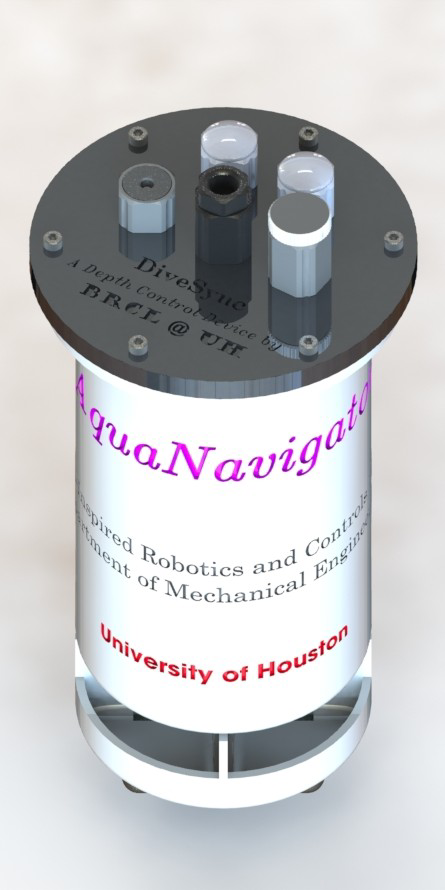
\includegraphics[height=3.1in]{Fig/ch2_bcd_cad_isometric.png}
    \end{minipage}
    \hfill
    \begin{minipage}{0.42\textwidth}
        \centering
        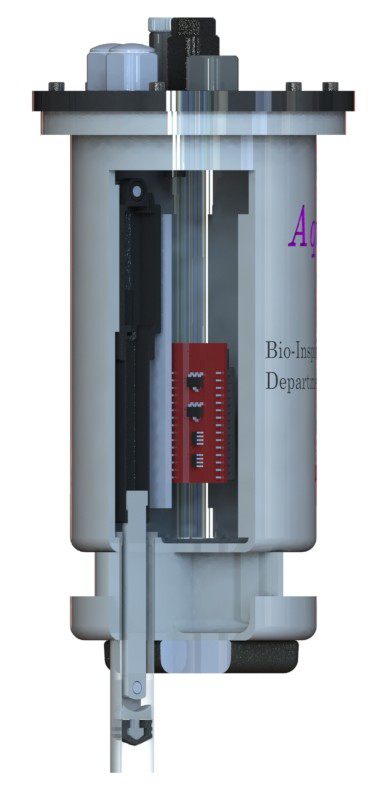
\includegraphics[height=3.1in]{Fig/ch2_bcd_cad_section.png}
    \end{minipage}
    \caption{Standalone BCD pressure-boundary and actuator layout.}
    \label{fig:ch2_bcd_cad}
\end{figure}

The cylindrical pressure boundary contains the actuator, piston assembly, electronics, and waterproof penetrations. The lower section provides space for balancing mass and mechanical support. This layout allows the device to be tuned near neutral buoyancy before closed-loop depth experiments. Developing the BCD as a standalone vertical-motion device also makes the modeling and testing process independent of the full robotic fish.

\section{Design of AquaNavigator}

AquaNavigator is designed as a bio-inspired robotic fish for underwater inspection and environmental monitoring experiments. The design methodology follows three parts: the caudal-fin propulsion system, the electronics and buoyancy enclosure, and the passive body covers that give the platform its fish-like shape. The design begins from tail-based propulsion because the robot's motion is generated by an oscillatory caudal-fin mechanism rather than by conventional propellers.

\subsection{Tail Propulsion and Steering}

The propulsion design is inspired by undulatory fish locomotion. The lateral displacement of a swimming body can be described using a traveling wave \cite{lighthill1969hydromechanics,Lighthill1971},
\begin{equation}
    y(x,t) = (c_1x+c_2x^2)\sin(kx+\omega t),
    \label{eq:ch2_design_wave}
\end{equation}
where $y$ is lateral displacement, $x$ is the position along the body, $c_1$ and $c_2$ define the amplitude envelope, $k$ is the body wave number, and $\omega$ is the oscillation frequency. For a robotic mechanism, the continuous body wave must be approximated by a finite number of rigid links. For a discretized body with link index $i$, the wave description can be written as
\begin{equation}
    \begin{aligned}
        y_i(x_i,t) &= (c_1x_i+c_2x_i^2)\sin(kx_i+\omega t), \\
        l_i &= \sqrt{(x_{i+1}-x_i)^2+(y_{i+1}-y_i)^2}.
    \end{aligned}
    \label{eq:ch2_discrete_wave}
\end{equation}
This representation motivates the use of at least two effective tail links if the robotic fish is to approximate an undulatory wave rather than a single rigid oscillating foil.

An open-chain two-joint tail could produce this motion by controlling two motors and their relative phase. However, a compact underwater robot benefits from fewer actuators, simpler waterproofing, and simpler low-level control. AquaNavigator therefore uses a double-slider-crank (DSC) mechanism that produces a two-link wave-like motion using one rotary input and a mechanically fixed phase shift \cite{Zuo2021,Masood2025Pipeline}. The phase relationship is selected through the mechanism geometry rather than enforced by two synchronized motors.

The mechanism is shown in Fig.~\ref{fig:ch2_dsc_action}. The motor drives two slider-crank stages in series so that the tail links move with a prescribed phase difference. Because the phase difference is set mechanically, the tail can generate an oscillatory wave-like motion without requiring two independently synchronized motors. This is useful for a compact underwater robot because it reduces actuator count and simplifies low-level propulsion commands. The tradeoff is that the tail kinematics are mostly fixed by the mechanism geometry, so the controller regulates swimming behavior through tail frequency and steering bias rather than through arbitrary joint trajectories.

\begin{figure}[t]
    \centering
    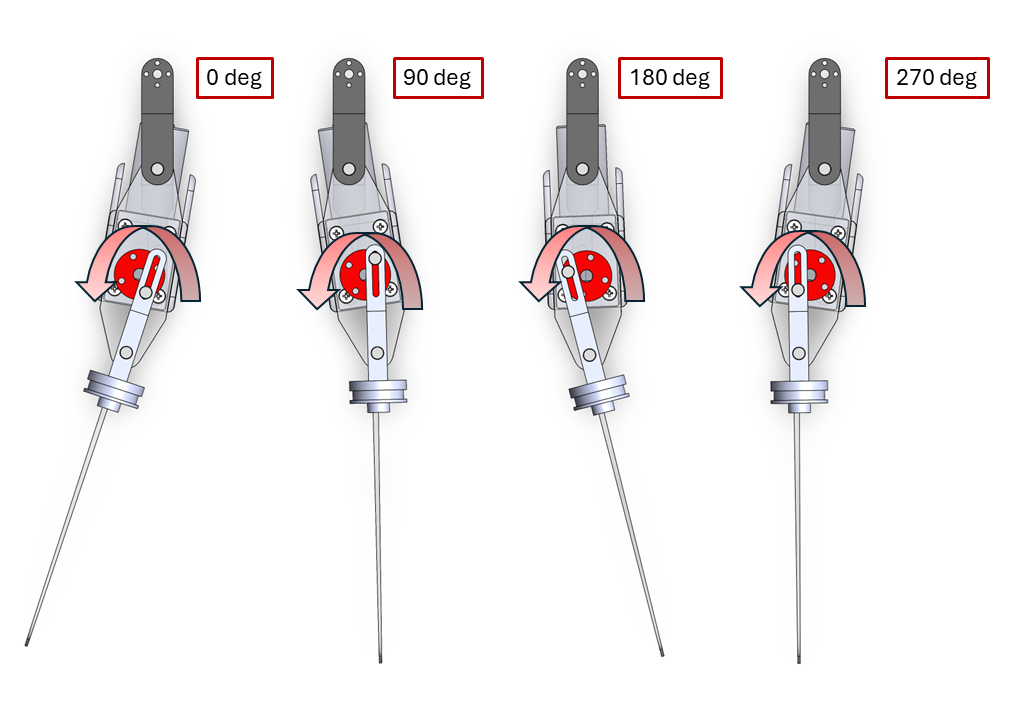
\includegraphics[width=0.86\textwidth]{Fig/ch2_dsc_action.png}
    \caption{Double-slider-crank tail mechanism at four crank positions.}
    \label{fig:ch2_dsc_action}
\end{figure}

Steering is achieved by rotating the complete tail-thrust module with a servo motor, as shown in Fig.~\ref{fig:ch2_tail_servo}. The servo changes the tail-bias angle, which changes the direction of the average thrust generated by the DSC mechanism. This creates yaw motion and allows the robot to track visual or mission-level commands. The same design also explains why the platform is underactuated: lateral motion is not directly commanded by a separate thruster, but appears through hydrodynamic coupling and tail-generated yaw.

\begin{figure}[t]
    \centering
    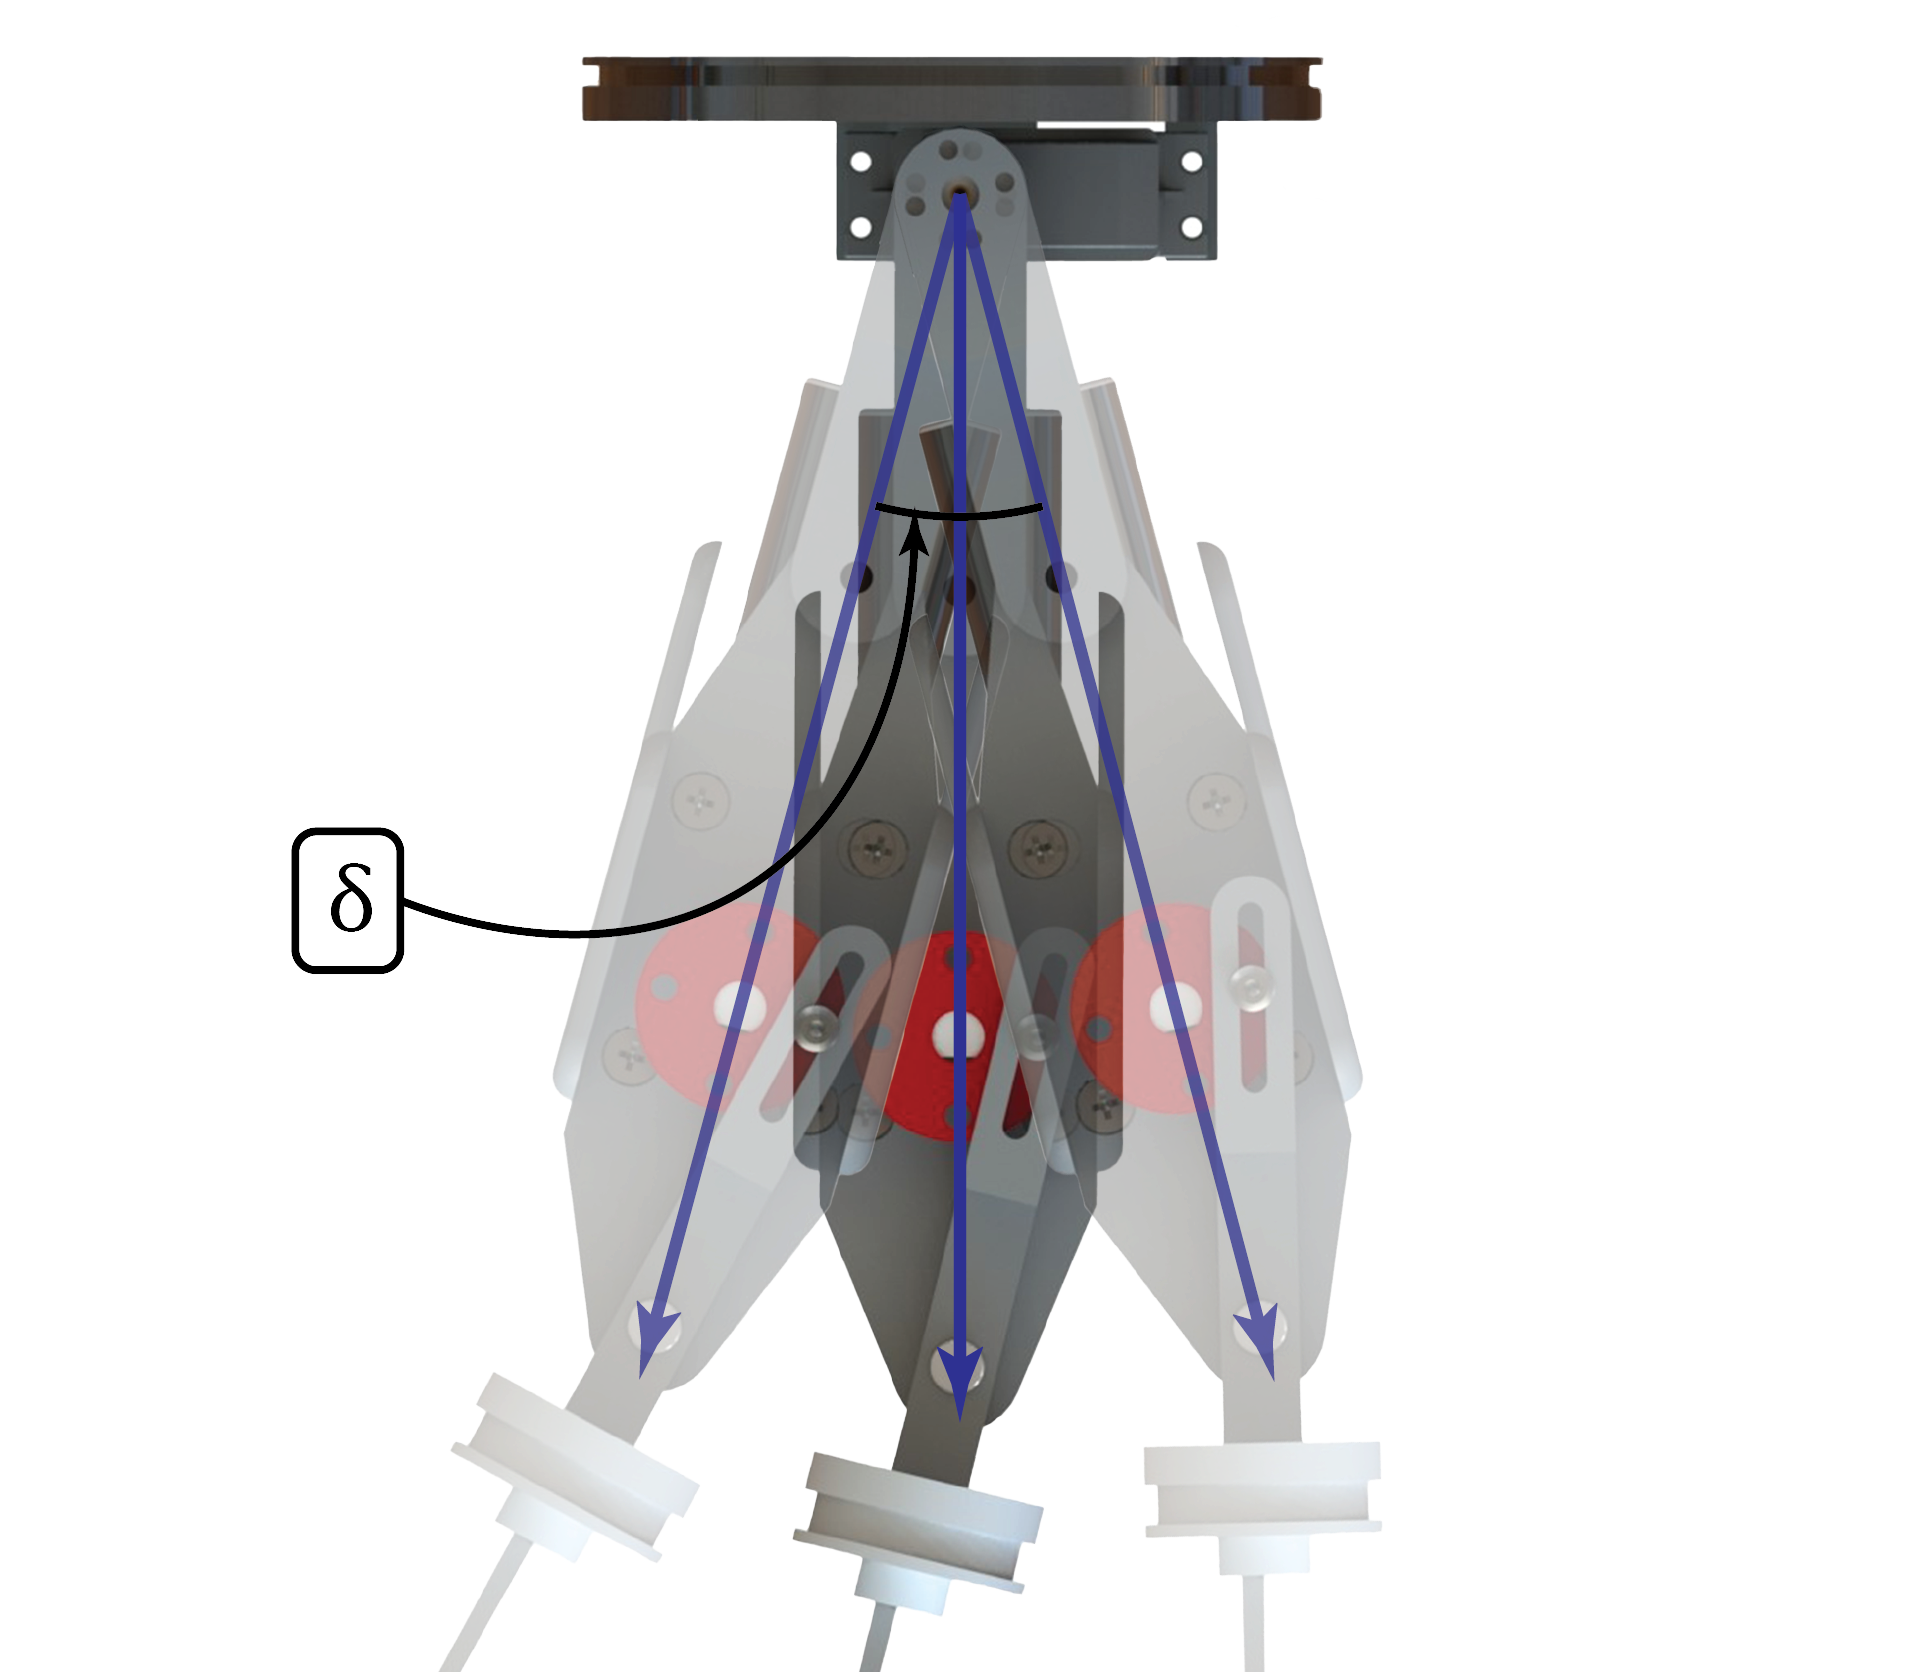
\includegraphics[width=0.62\textwidth]{Fig/ch2_tail_servo.png}
    \caption{Tail-bias servo for redirecting DSC tail thrust.}
    \label{fig:ch2_tail_servo}
\end{figure}

\subsection{Electronics, Sensing, and Enclosure Integration}

The electronics enclosure is the main integration volume of AquaNavigator. It houses the microcontroller, power distribution, battery connection, motor interfaces, camera connection, sensor interfaces, and buoyancy hardware. The depth-control mechanism is based on the piston-cylinder BCD concept described in the previous section. The linear actuator is placed inside the watertight enclosure so that the actuator body does not require a separate ingress-protection design.

The camera is mounted near the front of the robot and tilted downward from the horizontal direction so that pipeline-like features can appear in the field of view during swimming. The passive head cover includes an optical opening for the camera. The enclosure uses O-ring sealing and waterproof penetrators for wiring. The externally exposed servo motor and tail DC motor are individually sealed for operation in water. The body covers are shaped to give the robot a fish-like profile and to reduce drag relative to an exposed mechanical frame.

Figure~\ref{fig:ch2_aquanavigator_cad} shows the system-level layout. The tail section contains the DSC mechanism and tail-bias servo. The main enclosure carries the electronics, battery, camera interface, and sensor payloads. The front cover provides the fish-like body shape and the camera opening.

\begin{figure}[t]
    \centering
    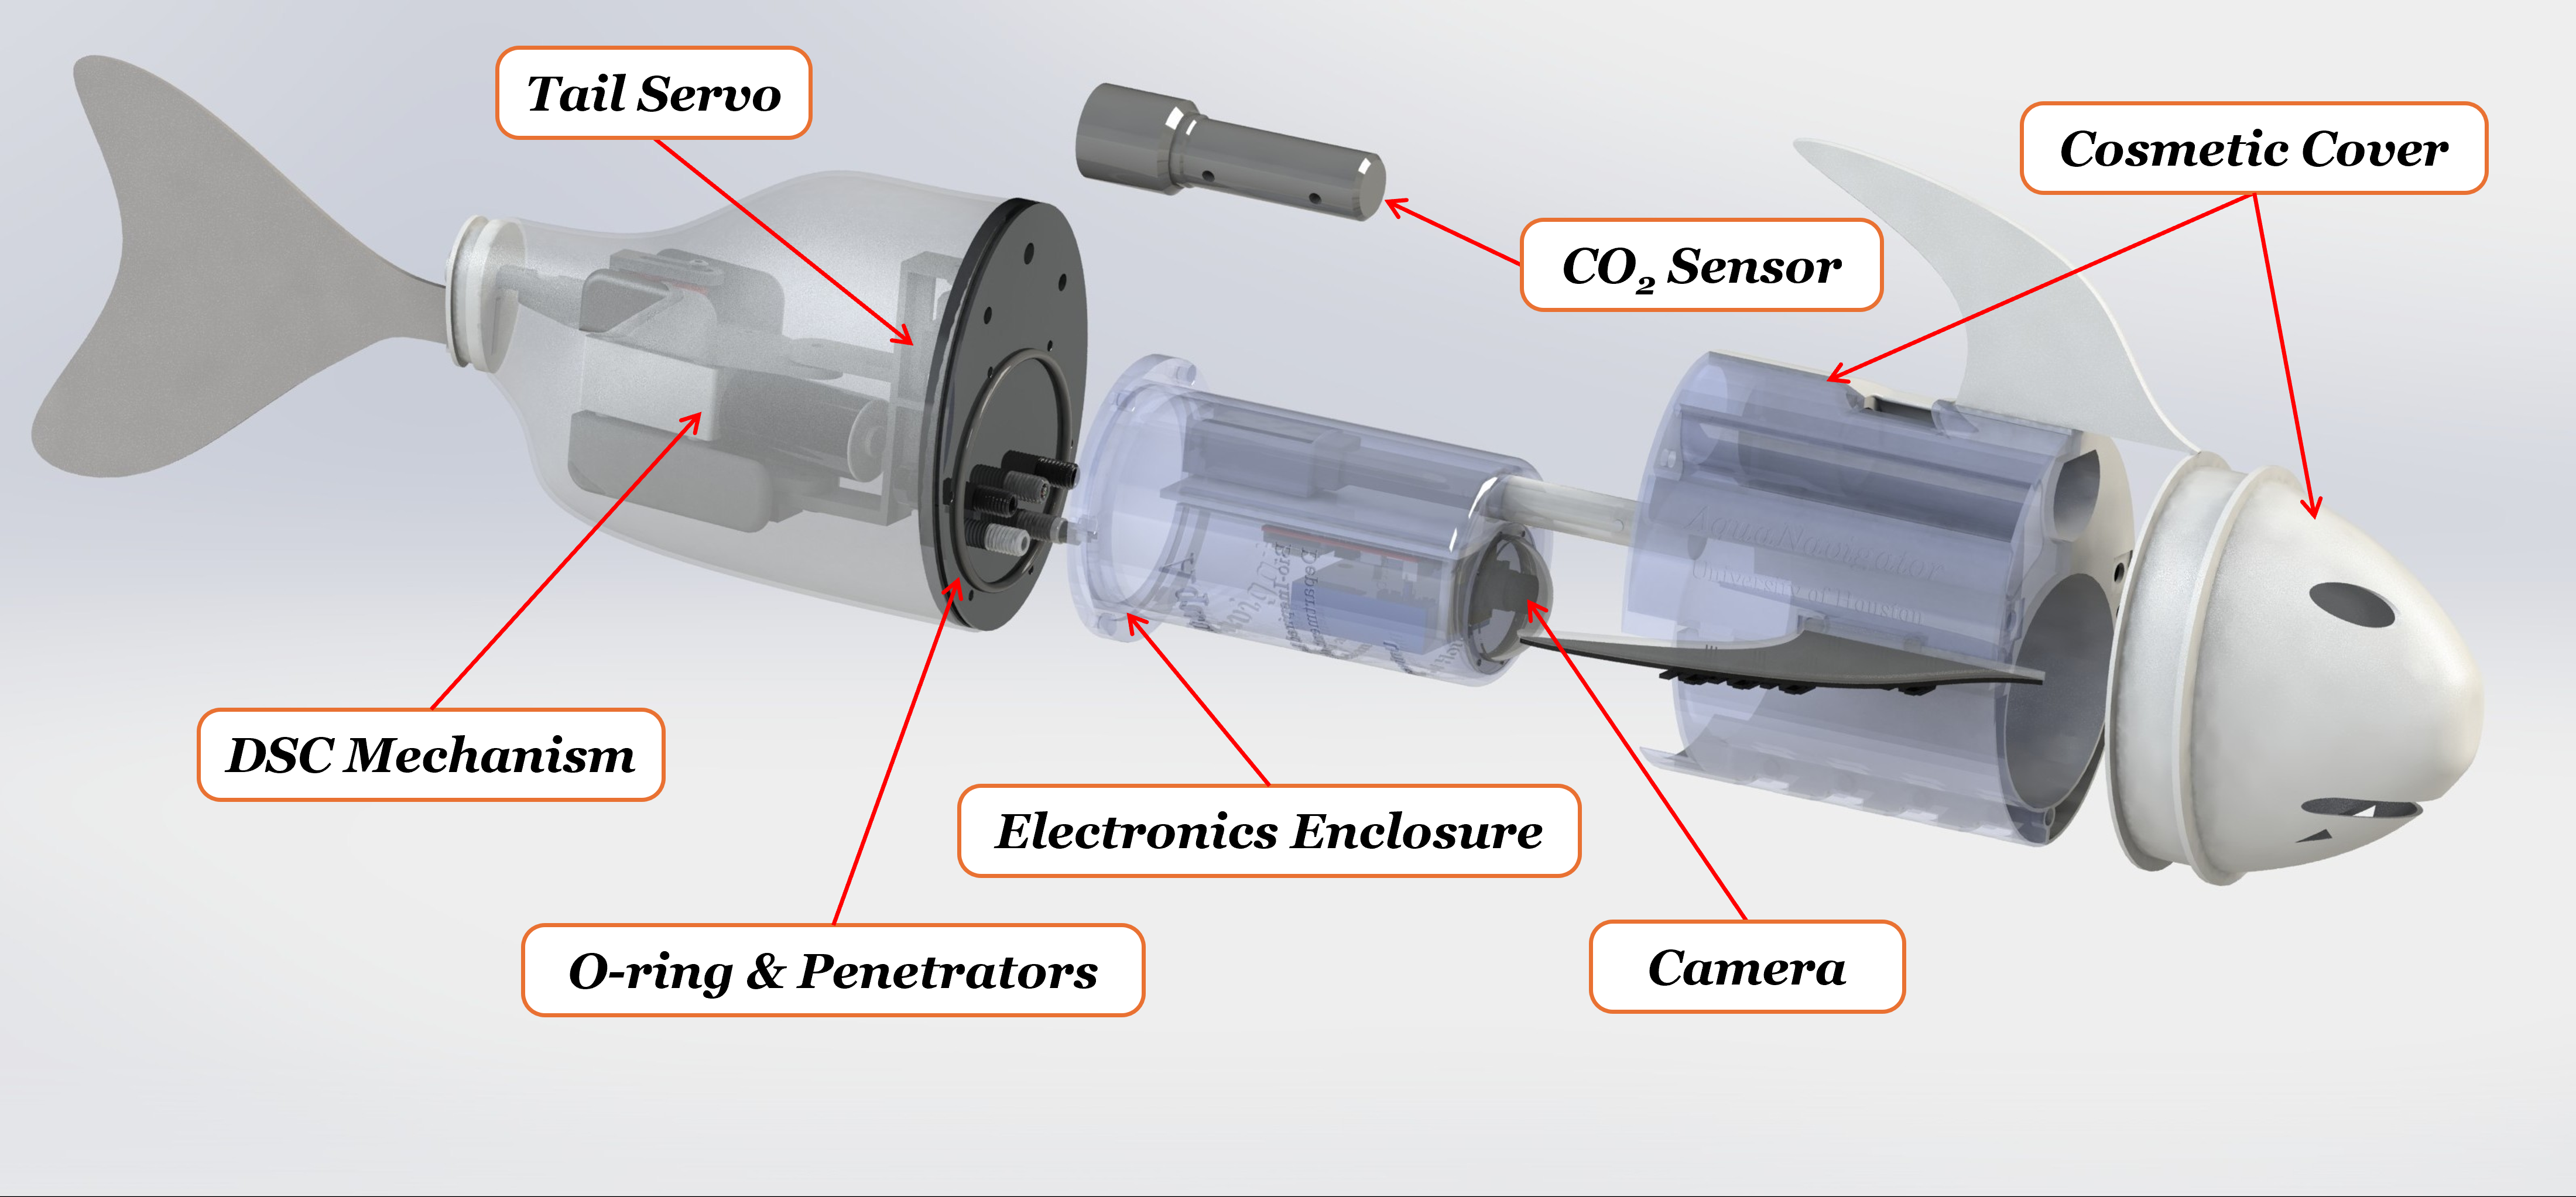
\includegraphics[width=\textwidth]{Fig/ch2_aquanavigator_cad.png}
    \caption{AquaNavigator exploded CAD layout and payload interfaces.}
    \label{fig:ch2_aquanavigator_cad}
\end{figure}

Table~\ref{tab:ch2_aquanavigator_specs} lists the platform specifications used in the current thesis experiments. The values should be interpreted as prototype-level specifications for controlled laboratory and pool validation.

\begin{table}[t]
    \centering
    \caption{Prototype AquaNavigator specifications for thesis experiments.}
    \label{tab:ch2_aquanavigator_specs}
    \begin{tabular}{lll}
        \hline
        Parameter & Value & Unit \\
        \hline
        Length & 0.67 & m \\
        Mass & 2.5 & kg \\
        Swimming speed & 0.2 & m/s \\
        Body-length speed & 0.3 & BL/s \\
        Swimming style & Carangiform & -- \\
        Nominal battery life & 40 & min \\
        Main onboard sensors & Camera, IMU, depth, NDIR \mbox{CO$_2$} & -- \\
        \hline
    \end{tabular}
\end{table}

\section{Modeling of the BCD and Robotic Fish}

The modeling framework has two parts. The first part describes the BCD as a coupled buoyancy and actuator system. The second part describes AquaNavigator as a tail-actuated planar robotic fish. The BCD model supports depth-control design, while the robotic-fish model supports simulation, controller tuning, and interpretation of pipeline-tracking experiments.

\subsection{Buoyancy-Device Force Balance}

The BCD model begins with the free-body diagram in Fig.~\ref{fig:ch2_bcd_schematic}. Let $x_d$ denote the device depth displacement relative to a neutral reference position, with positive $x_d$ taken downward. The device mass is denoted by $m$, the surrounding water density by $\rho_w$, and the fixed displaced volume at neutral buoyancy by $V_s$. The piston changes the displaced volume by a signed dynamic component $V_d$. The hydrodynamic drag in the vertical direction is approximated as linear with coefficient $c_d$.

\begin{figure}[t]
    \centering
    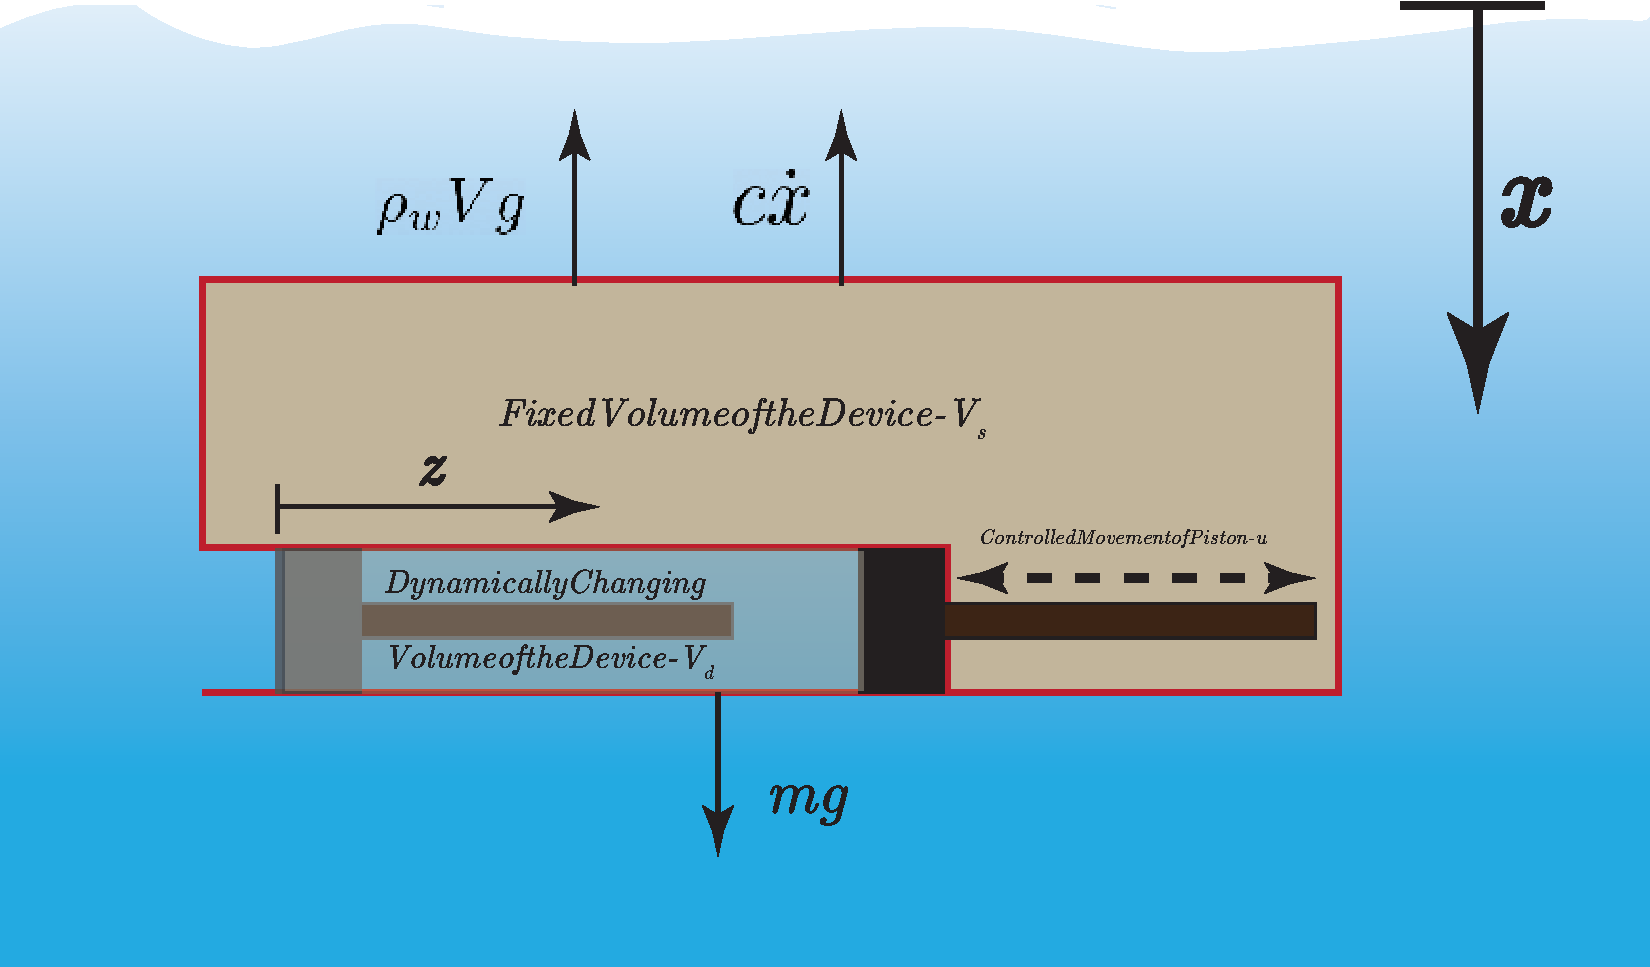
\includegraphics[width=0.78\textwidth]{Fig/ch2_bcd_schematic.pdf}
    \caption{BCD free-body model near neutral buoyancy.}
    \label{fig:ch2_bcd_schematic}
\end{figure}

The total displaced volume is
\begin{equation}
    V = V_s + V_d .
    \label{eq:ch2_bcd_total_volume}
\end{equation}
At the nominal neutral-buoyancy condition,
\begin{equation}
    m = \rho_w V_s .
    \label{eq:ch2_bcd_neutral}
\end{equation}
The vertical equation of motion can then be written as
\begin{equation}
    m\ddot{x}_d = mg - \rho_w (V_s + V_d)g - c_d\dot{x}_d .
    \label{eq:ch2_bcd_force_balance}
\end{equation}
Using Eq.~\eqref{eq:ch2_bcd_neutral}, the neutral weight and buoyancy terms cancel and the depth dynamics reduce to
\begin{equation}
    \ddot{x}_d + \frac{c_d}{m}\dot{x}_d
    = -\frac{\rho_w g}{m}V_d .
    \label{eq:ch2_bcd_depth_vd}
\end{equation}
The sign of $V_d$ depends on the chosen positive piston direction. In the implementation, the actuator calibration maps command direction to the desired increase or decrease of buoyancy. For modeling, it is convenient to define an effective piston displacement $x_p$ such that
\begin{equation}
    V_d = A_p x_p, \qquad A_p = \pi r_p^2 ,
    \label{eq:ch2_bcd_piston_volume}
\end{equation}
where $A_p$ is the piston area and $r_p$ is the piston radius. The piston notation is shown in Fig.~\ref{fig:ch2_bcd_piston}.

\begin{figure}[t]
    \centering
    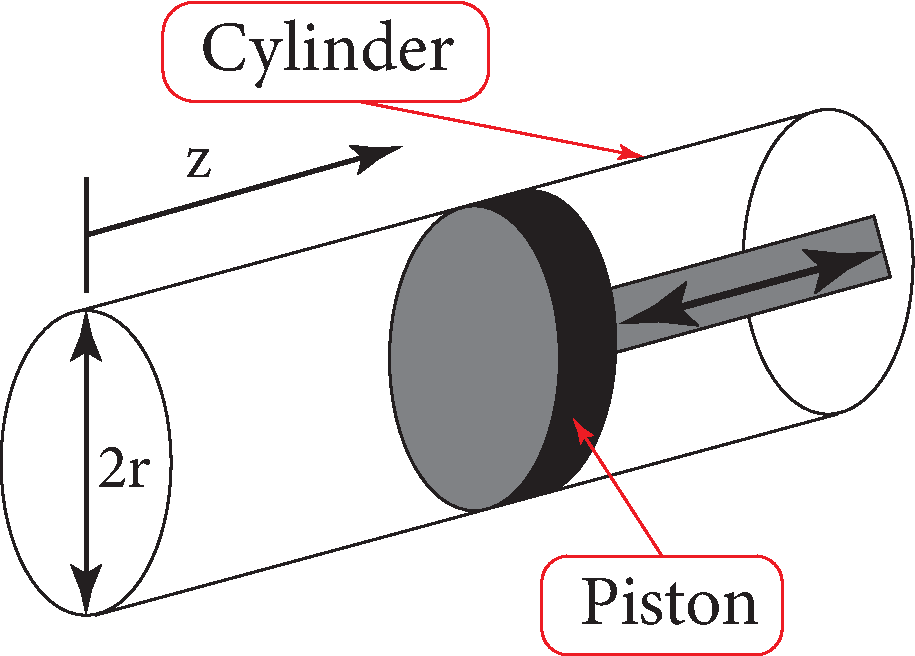
\includegraphics[width=0.48\textwidth]{Fig/ch2_bcd_piston.pdf}
    \caption{Piston-cylinder notation for BCD volume change.}
    \label{fig:ch2_bcd_piston}
\end{figure}

Substituting Eq.~\eqref{eq:ch2_bcd_piston_volume} into Eq.~\eqref{eq:ch2_bcd_depth_vd} gives the basic second-order vertical-motion model,
\begin{equation}
    \ddot{x}_d + \frac{c_d}{m}\dot{x}_d
    = -\frac{\rho_w g A_p}{m}x_p .
    \label{eq:ch2_bcd_depth_xp}
\end{equation}
This equation captures the main physical effect of the BCD: piston displacement changes the displaced volume and therefore creates vertical acceleration. It also shows why the neutral operating point is delicate. If a small piston offset or mass-balancing error creates a nonzero net buoyancy, the device will continue to move unless drag and control action counteract the imbalance.

\subsection{Pressure-Coupled Actuator Model}

The BCD model treats the piston actuator as part of the plant rather than as an ideal position source \cite{Masood2026ESCBCD}. This is important because the actuator is not only moving a piston in air. It is coupled to hydrostatic pressure, internal chamber pressure, friction, backlash, dead-zone behavior, and voltage limits. The motor-side electrical model can be written as
\begin{equation}
    R_a i_a + L_a \dot{i}_a + K_b'\dot{x}_p = u_a ,
    \label{eq:ch2_actuator_electrical}
\end{equation}
where $R_a$ is the armature resistance, $L_a$ is the armature inductance, $i_a$ is the armature current, $K_b'$ is the back-emf constant referred to piston velocity, and $u_a$ is the applied actuator voltage. For the reduced model used in the control development, the armature inductance is neglected, so
\begin{equation}
    i_a = \frac{u_a - K_b'\dot{x}_p}{R_a}.
    \label{eq:ch2_actuator_current}
\end{equation}

The piston-force balance is modeled as
\begin{equation}
    m_l\ddot{x}_p = -f_l\dot{x}_p + K_f i_a + F_p ,
    \label{eq:ch2_piston_force}
\end{equation}
where $m_l$ is the equivalent moving mass of the actuator-piston assembly, $f_l$ is the equivalent viscous damping coefficient, $K_f$ is the actuator force constant, and $F_p$ represents pressure-induced loading on the piston. If pressure terms are temporarily ignored, substituting Eq.~\eqref{eq:ch2_actuator_current} into Eq.~\eqref{eq:ch2_piston_force} gives
\begin{equation}
    \ddot{x}_p =
    -\frac{R_a f_l + K_f K_b'}{m_l R_a}\dot{x}_p
    + \frac{K_f}{m_l R_a}u_a .
    \label{eq:ch2_basic_actuator_model}
\end{equation}
Equivalently, the reduced actuator model can be written as
\begin{equation}
    \tau \ddot{x}_p + \dot{x}_p = K_l u_a ,
    \label{eq:ch2_tau_actuator}
\end{equation}
where
\begin{equation}
    \tau = \frac{m_l R_a}{R_a f_l + K_f K_b'}, \qquad
    K_l = \frac{K_f}{R_a f_l + K_f K_b'} .
    \label{eq:ch2_tau_kl}
\end{equation}

The pressure-coupled model adds two effects that are important for underwater operation. First, the external hydrostatic pressure changes with depth and loads the piston. Second, the sealed internal volume changes as the piston moves, creating an opposing pressure term. With these effects included, the piston dynamics take the form
\begin{equation}
    \ddot{x}_p =
    -\frac{1}{\tau}\dot{x}_p
    + \frac{K_l}{\tau}u_a
    + \frac{A_p \rho_w g}{m_l}x_d
    - \frac{A_p^2 P_s}{m_l V_{se}}x_p ,
    \label{eq:ch2_pressure_coupled_actuator}
\end{equation}
where $P_s$ is the equilibrium internal chamber pressure and $V_{se}$ is the equilibrium enclosed chamber volume. This model shows the coupling between actuator motion and depth. Depth changes the external pressure acting on the piston, while piston motion changes the device volume and therefore the vertical acceleration.

Combining Eqs.~\eqref{eq:ch2_bcd_depth_xp} and \eqref{eq:ch2_pressure_coupled_actuator} gives a fourth-order BCD model with state vector
\begin{equation}
    \mathbf{x}_b =
    \begin{bmatrix}
        x_d & \dot{x}_d & x_p & \dot{x}_p
    \end{bmatrix}^T .
    \label{eq:ch2_bcd_state}
\end{equation}
A compact state-space form is
\begin{equation}
    \dot{\mathbf{x}}_b =
    \begin{bmatrix}
        0 & 1 & 0 & 0 \\
        0 & -\frac{c_d}{m} & -\frac{\rho_w g A_p}{m} & 0 \\
        0 & 0 & 0 & 1 \\
        \frac{A_p \rho_w g}{m_l} & 0 &
        -\frac{A_p^2 P_s}{m_l V_{se}} & -\frac{1}{\tau}
    \end{bmatrix}
    \mathbf{x}_b
    +
    \begin{bmatrix}
        0 \\ 0 \\ 0 \\ \frac{K_l}{\tau}
    \end{bmatrix}u_a .
    \label{eq:ch2_bcd_statespace}
\end{equation}
The model in Eq.~\eqref{eq:ch2_bcd_statespace} is the main BCD model used by this dissertation to explain why depth regulation is a constraint-sensitive problem. The controller must respect piston stroke limits, actuator voltage limits, and the instability near neutral buoyancy. These issues are treated in Chapter~3, where model validation and control design are presented.

\subsection{AquaNavigator Dynamic Model}

The robotic-fish dynamic model is derived in two steps. First, the force generated by the flapping DSC tail is estimated. Second, the planar rigid-body dynamics of the robot are written using surge, sway, and yaw motion. The model is not intended to represent every fluid-structure interaction around the fish. It provides a tractable representation for simulation, controller design, and interpretation of the experimental behavior.

The coordinate frames used for the planar model are shown in Fig.~\ref{fig:ch2_robot_frames}:
\begin{itemize}
\item[$\{W\}$] Fixed to the laboratory or simulation environment
\item[$\{B\}$] Attached to the center of mass of the robotic fish
\item[$\{D\}$] Attached to the tail mechanism
\item[$\{CF\}$] Attached to the tail/fin section used for force estimation
\end{itemize}

\begin{figure}[t]
    \centering
    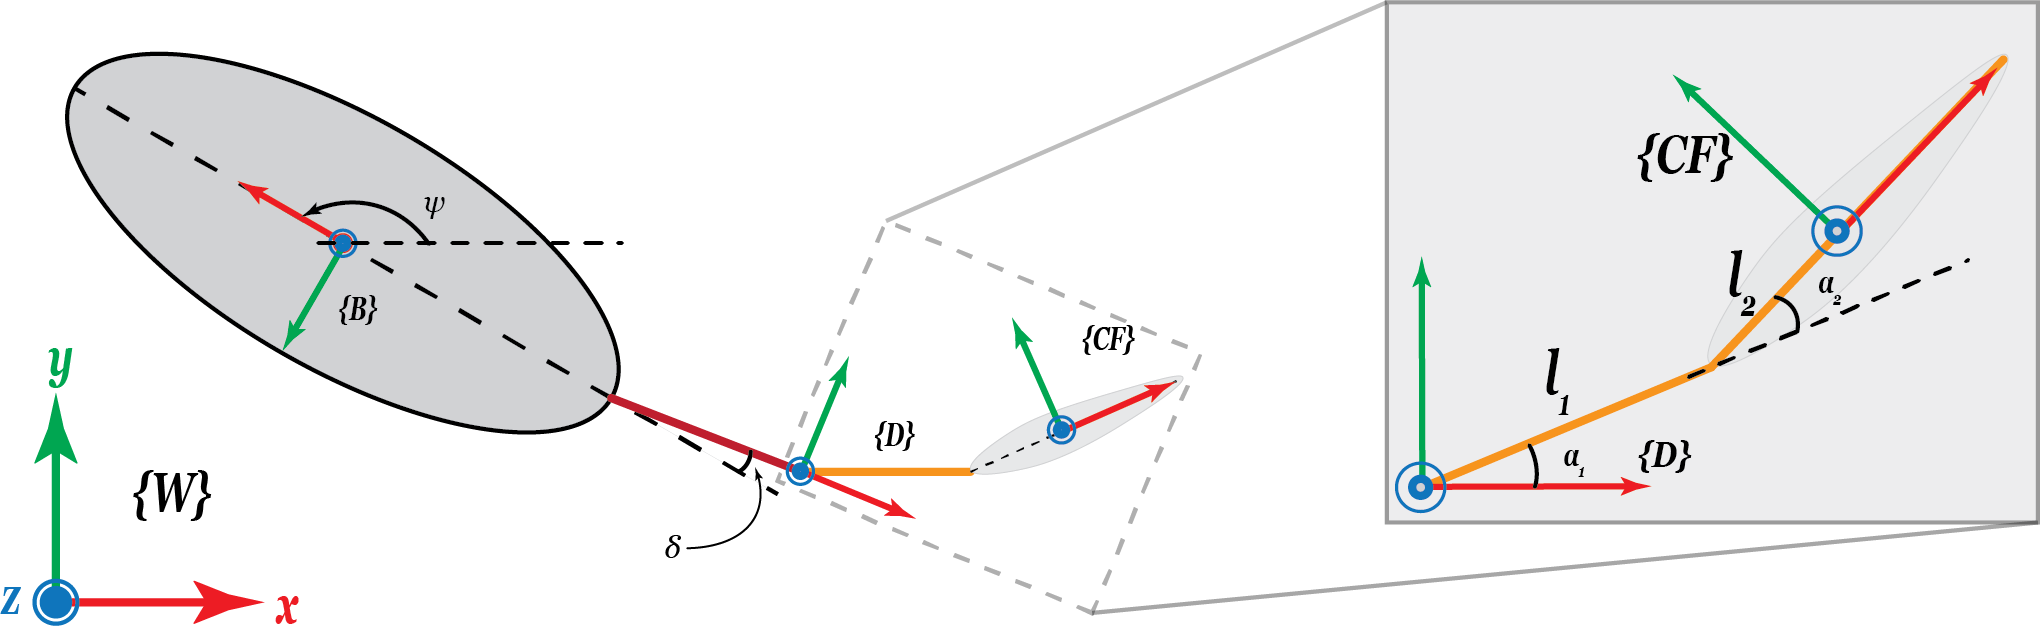
\includegraphics[width=\textwidth]{Fig/ch2_robot_frames.png}
    \caption{AquaNavigator frames for propulsion and planar dynamics.}
    \label{fig:ch2_robot_frames}
\end{figure}

The world frame is placed on the water-surface plane, with its $z$-axis pointing downward. For tank experiments, its origin can be chosen at a convenient fixed point in the camera view. The body frame uses the robot heading direction as its $x$-axis and the lateral direction as its $y$-axis. The DSC frame is located at the tail mechanism joint associated with the link $l_0$, and the caudal-fin frame is placed at the quarter-chord point of the fin. The caudal-fin frame is used because the elongated-body force approximation is evaluated from the normal and tangential velocities at that point.

The following assumptions are used in the planar model:
\begin{enumerate}
\item Roll and pitch motion are assumed to be negligible because the robot is balanced so that it remains upright during nominal swimming.
\item The robotic fish is treated as an underactuated nonholonomic system. It does not generate independent lateral thrust; sway appears through hydrodynamic coupling.
\item The body-fixed frame is located at the center of mass, with surge velocity $u$, sway velocity $v$, and yaw rate $r$.
\item The surrounding fluid is treated using a simplified hydrodynamic approximation, so the model focuses on dominant inertial and drag effects rather than full CFD.
\item The caudal-fin force is estimated using an elongated-body-theory approximation, with the tail treated as a stiff, low-frequency oscillating structure.
\end{enumerate}

\subsubsection{Tail Kinematics and Thrust Estimation}

Let $\alpha_1$ and $\alpha_2$ denote the angular positions of the two effective tail links. For the DSC mechanism, the link motion is approximated by
\begin{equation}
    \begin{aligned}
        \alpha_1(t) &= A_1 \sin(\omega t), \\
        \alpha_2(t) &= A_2 \sin(\omega t+\phi_{dsc}),
    \end{aligned}
    \label{eq:ch2_dsc_angles}
\end{equation}
where $A_1$ and $A_2$ are link angular amplitudes and $\phi_{dsc}$ is the fixed phase difference set by the mechanism geometry. The phase difference is not an online control input in the present prototype. The main propulsion command is the tail oscillation frequency $\omega$, while the steering command is the tail-bias angle $\delta$. Following the DSC mechanism design, $\phi_{dsc}$ is taken as a fixed phase difference.

If the quarter-chord point of the caudal fin is used as the force-evaluation point, its position in the DSC frame can be approximated as
\begin{equation}
    \begin{aligned}
        x_{qc} &= l_1\cos(\alpha_1) + l_2\cos(\alpha_2), \\
        y_{qc} &= l_1\sin(\alpha_1) + l_2\sin(\alpha_2), \\
        \dot{x}_{qc} &= -l_1\omega\sin(\alpha_1)-l_2\omega\sin(\alpha_2), \\
        \dot{y}_{qc} &= l_1\omega\cos(\alpha_1)+l_2\omega\cos(\alpha_2),
    \end{aligned}
    \label{eq:ch2_qc_position}
\end{equation}
where $l_1$ and $l_2$ are effective link lengths. The corresponding normal and tangential velocity components in the caudal-fin frame are
\begin{equation}
    \begin{aligned}
        V_{\parallel} &=
        -\dot{x}_{qc}\sin(\alpha_2) + \dot{y}_{qc}\cos(\alpha_2), \\
        V_{\perp} &=
        \dot{x}_{qc}\cos(\alpha_2) + \dot{y}_{qc}\sin(\alpha_2).
    \end{aligned}
    \label{eq:ch2_cf_velocity}
\end{equation}
Using the elongated-body approximation adopted in the pipeline-tracking model \cite{Wang2013,Lighthill1971,Masood2025Pipeline}, the tail-generated force in the DSC frame is written in terms of the normal and tangential velocity components as
\begin{equation}
    {}^{D}\mathbf{F}
    =
    \frac{1}{2}m_i V_{\perp}^{2}\hat{\mathbf{m}}
    - m_i V_{\perp}V_{\parallel}\hat{\mathbf{n}}
    + m_i L\dot{V}_{\perp}\hat{\mathbf{n}},
    \label{eq:ch2_tail_force_d}
\end{equation}
where $m_i$ is the virtual mass per unit length, $L$ is an effective body length, and $\hat{\mathbf{m}}$ and $\hat{\mathbf{n}}$ are the tangential and normal unit directions used in the tail-force approximation. The virtual mass per unit length is represented as
\begin{equation}
    m_i = \frac{1}{4}\pi\rho_w h^2 ,
    \label{eq:ch2_virtual_mass}
\end{equation}
where $h$ is the submerged body height used in the elongated-body approximation. The effective length $L$ is computed from the measured body and tail geometry of the prototype. The tail-bias angle $\delta$ rotates the generated force into the body frame:
\begin{equation}
    {}^{B}\mathbf{F}
    =
    \begin{bmatrix}
        F_x \\ F_y
    \end{bmatrix}
    =
    \begin{bmatrix}
        \cos\delta & -\sin\delta \\
        \sin\delta & \cos\delta
    \end{bmatrix}
    {}^{D}\mathbf{F}.
    \label{eq:ch2_tail_force_body}
\end{equation}
The resulting yaw moment about the body center is expressed as
\begin{equation}
    F_{\theta}
    =
    -\left((L-d_0)\cos\delta\right)F_y
    + (l_0+l_1+l_2)\sin\delta\,F_x ,
    \label{eq:ch2_yaw_moment}
\end{equation}
where $d_0$ and $l_0$ are geometry parameters associated with the body and tail-module placement.

\subsubsection{Planar Rigid-Body Dynamics}

The planar swimming model treats AquaNavigator as an underactuated surface or near-surface vehicle with surge, sway, and yaw dynamics. Let
\begin{equation}
    \boldsymbol{\nu} =
    \begin{bmatrix}
        u & v & r
    \end{bmatrix}^T
    \label{eq:ch2_body_velocity}
\end{equation}
denote the body-frame velocity vector, where $u$ is surge velocity, $v$ is sway velocity, and $r$ is yaw rate. The general rigid-body form is
\begin{equation}
    \mathbf{M}\dot{\boldsymbol{\nu}}
    + \mathbf{C}(\boldsymbol{\nu})\boldsymbol{\nu}
    + \mathbf{D}\boldsymbol{\nu}
    =
    \mathbf{F},
    \label{eq:ch2_general_fish_model}
\end{equation}
where $\mathbf{M}$ is the inertia and added-mass matrix, $\mathbf{C}$ is the Coriolis and centripetal matrix, $\mathbf{D}$ is the damping matrix, and
\begin{equation}
    \mathbf{F} =
    \begin{bmatrix}
        F_x & F_y & F_{\theta}
    \end{bmatrix}^T
    \label{eq:ch2_fish_force_vector}
\end{equation}
is the generalized force vector generated primarily by the tail mechanism.

Using the simplified form from the pipeline-tracking model, the planar equations can be written as
\begin{equation}
    \begin{aligned}
        (m+k_{11}m)\dot{u}
        &= F_x + (m+k_{22}m)vr - D_u u, \\
        (m+k_{22}m)\dot{v}
        &= F_y + (m+k_{11}m)ur - D_v v, \\
        (I+k_{55}I)\dot{r}
        &= F_{\theta} - (k_{22}m-k_{11}m)uv - D_r r .
    \end{aligned}
    \label{eq:ch2_planar_eom}
\end{equation}
Here $m$ is the robot mass, $I$ is the yaw moment of inertia, $k_{11}$, $k_{22}$, and $k_{55}$ are added-mass coefficients, and $D_u$, $D_v$, and $D_r$ are lumped damping coefficients. The added-mass approximation treats the body as a prolate ellipsoid with semi-axes $a$, $b$, and $b$.

The added-mass coefficients are estimated using Lamb's $k$-factor representation,
\begin{equation}
    \begin{aligned}
        k_{11} &= \frac{\alpha_0}{2-\alpha_0}, \\
        k_{22} &= \frac{\beta_0}{2-\beta_0}, \\
        k_{55} &=
        \frac{e^4(\beta_0-\alpha_0)}
        {(2-e^2)\left(2e^2-(2-e^2)(\beta_0-\alpha_0)\right)},
    \end{aligned}
    \label{eq:ch2_added_mass_coefficients}
\end{equation}
where
\begin{equation}
    \begin{aligned}
        \alpha_0 &=
        \frac{2(1-e^2)}{e^3}
        \left(\frac{1}{2}\ln\frac{1+e}{1-e}-e\right), \\
        \beta_0 &=
        \frac{1}{e^2}
        -\frac{1-e^2}{2e^3}\ln\frac{1+e}{1-e},
    \end{aligned}
    \label{eq:ch2_lamb_factors}
\end{equation}
and
\begin{equation}
    e = \sqrt{1-\frac{b^2}{a^2}}
    \label{eq:ch2_eccentricity}
\end{equation}
is the ellipsoid eccentricity. The ellipsoid approximation is chosen so that the body mass and yaw inertia are consistent with
\begin{equation}
    m = \frac{4}{3}\pi\rho_wab^2, \qquad
    I = \frac{4}{15}\pi\rho_wab^2(a^2+b^2).
    \label{eq:ch2_ellipsoid_mass_inertia}
\end{equation}
For AquaNavigator, this approximation requires care because some body cavities and passive covers can fill with water during operation. The effective submerged geometry, not only the dry mass, determines the added-mass approximation.

The damping matrix is written as
\begin{equation}
    \mathbf{D} =
    \begin{bmatrix}
        D_u & 0 & 0 \\
        0 & D_v & 0 \\
        0 & 0 & D_r
    \end{bmatrix}
    =
    \begin{bmatrix}
        \frac{\partial F_x}{\partial u} & 0 & 0 \\
        0 & \frac{\partial F_y}{\partial v} & 0 \\
        0 & 0 & \frac{\partial F_{\theta}}{\partial r}
    \end{bmatrix}.
    \label{eq:ch2_damping_matrix}
\end{equation}
The nonlinear drag components can be approximated as
\begin{equation}
    \begin{aligned}
        F_{D_u} &= \frac{1}{2}\rho_w A_u C_u |u|u, \\
        F_{D_v} &= \frac{1}{2}\rho_w A_v C_v |v|v, \\
        F_{D_r} &= C_r |r|r,
    \end{aligned}
    \label{eq:ch2_drag_forces}
\end{equation}
where $A_u$, $A_v$, and $A_r$ are reference areas and $C_u$, $C_v$, and $C_r$ are drag coefficients. A local linear damping approximation can be taken around nominal velocities:
\begin{equation}
    \begin{aligned}
        D_u(\bar{u}) &=
        \left.\frac{\partial F_{D_u}}{\partial u}\right|_{u=\bar{u}}, \\
        D_v(\bar{v}) &=
        \left.\frac{\partial F_{D_v}}{\partial v}\right|_{v=\bar{v}}, \\
        D_r(\bar{r}) &=
        \left.\frac{\partial F_{D_r}}{\partial r}\right|_{r=\bar{r}}.
    \end{aligned}
    \label{eq:ch2_linear_damping}
\end{equation}
The resulting model is the basis for the simulation environment used in the pipeline-tracking work \cite{Masood2025Pipeline}. Table~\ref{tab:ch2_fish_model_parameters} lists the experimental and calculated parameters used in the model.

\begin{table}[t]
    \centering
    \caption{AquaNavigator model parameters and calculated coefficients.}
    \label{tab:ch2_fish_model_parameters}
    \begin{tabular}{lll}
        \hline
        Parameter & Value & Unit \\
        \hline
        \multicolumn{3}{c}{Experimental values} \\
        \hline
        $C_u$ & 0.05 & kg/s \\
        $C_v$ & 18.5 & kg/s \\
        $C_r$ & 0.49 & kg/s \\
        $k_f$ & 0.45 & N/A \\
        \hline
        \multicolumn{3}{c}{Calculated values} \\
        \hline
        $a$ & 0.234 & m \\
        $b$ & 0.065 & m \\
        $e$ & 0.96 & -- \\
        $\alpha_0$ & 0.173 & -- \\
        $\beta_0$ & 0.9135 & -- \\
        $k_{11}$ & 0.0947 & -- \\
        $k_{22}$ & 0.8408 & -- \\
        $k_{55}$ & 0.5587 & -- \\
        \hline
        \multicolumn{3}{c}{Geometry and body parameters} \\
        \hline
        $m_e$ & 4.14 & kg \\
        $I$ & 0.049 & kg m$^2$ \\
        $l_0$ & 0.06 & m \\
        $l_1$ & 0.1176 & m \\
        $l_2$ & 0.097 & m \\
        $d_0$ & 0.145 & m \\
        $A_1$ & 10 & deg \\
        $A_2$ & 13 & deg \\
        $\phi_{dsc}$ & 90 & deg \\
        \hline
    \end{tabular}
\end{table}

The model highlights the key design tradeoff of AquaNavigator. The DSC tail gives a compact propulsion system with a small actuator count, but the resulting motion is coupled and underactuated. Changing $\omega$ changes the magnitude and temporal structure of the thrust. Changing $\delta$ redirects the thrust and creates yaw. Sway motion is not directly actuated, and the robot body also experiences oscillatory motion because the propulsion mechanism is itself oscillatory. These modeling features are important for the later pipeline-tracking chapter, where visual measurements must be interpreted in the presence of tail-induced image motion and underactuated vehicle dynamics.

\section{Fabrication of the BCD and AquaNavigator}

The BCD was fabricated first as a standalone vertical-motion device. The enclosure, piston-cylinder assembly, top plate, balancing features, and actuator mount were manufactured and assembled before the device was used for depth-control experiments. The top plate carries the waterproof penetrations, electrical interface, and access hardware. The cylindrical body provides the sealed volume, while the lower piston-cylinder section changes the effective displaced volume. The fabricated device is shown in Fig.~\ref{fig:ch2_bcd_fabricated}.

\begin{figure}[t]
    \centering
    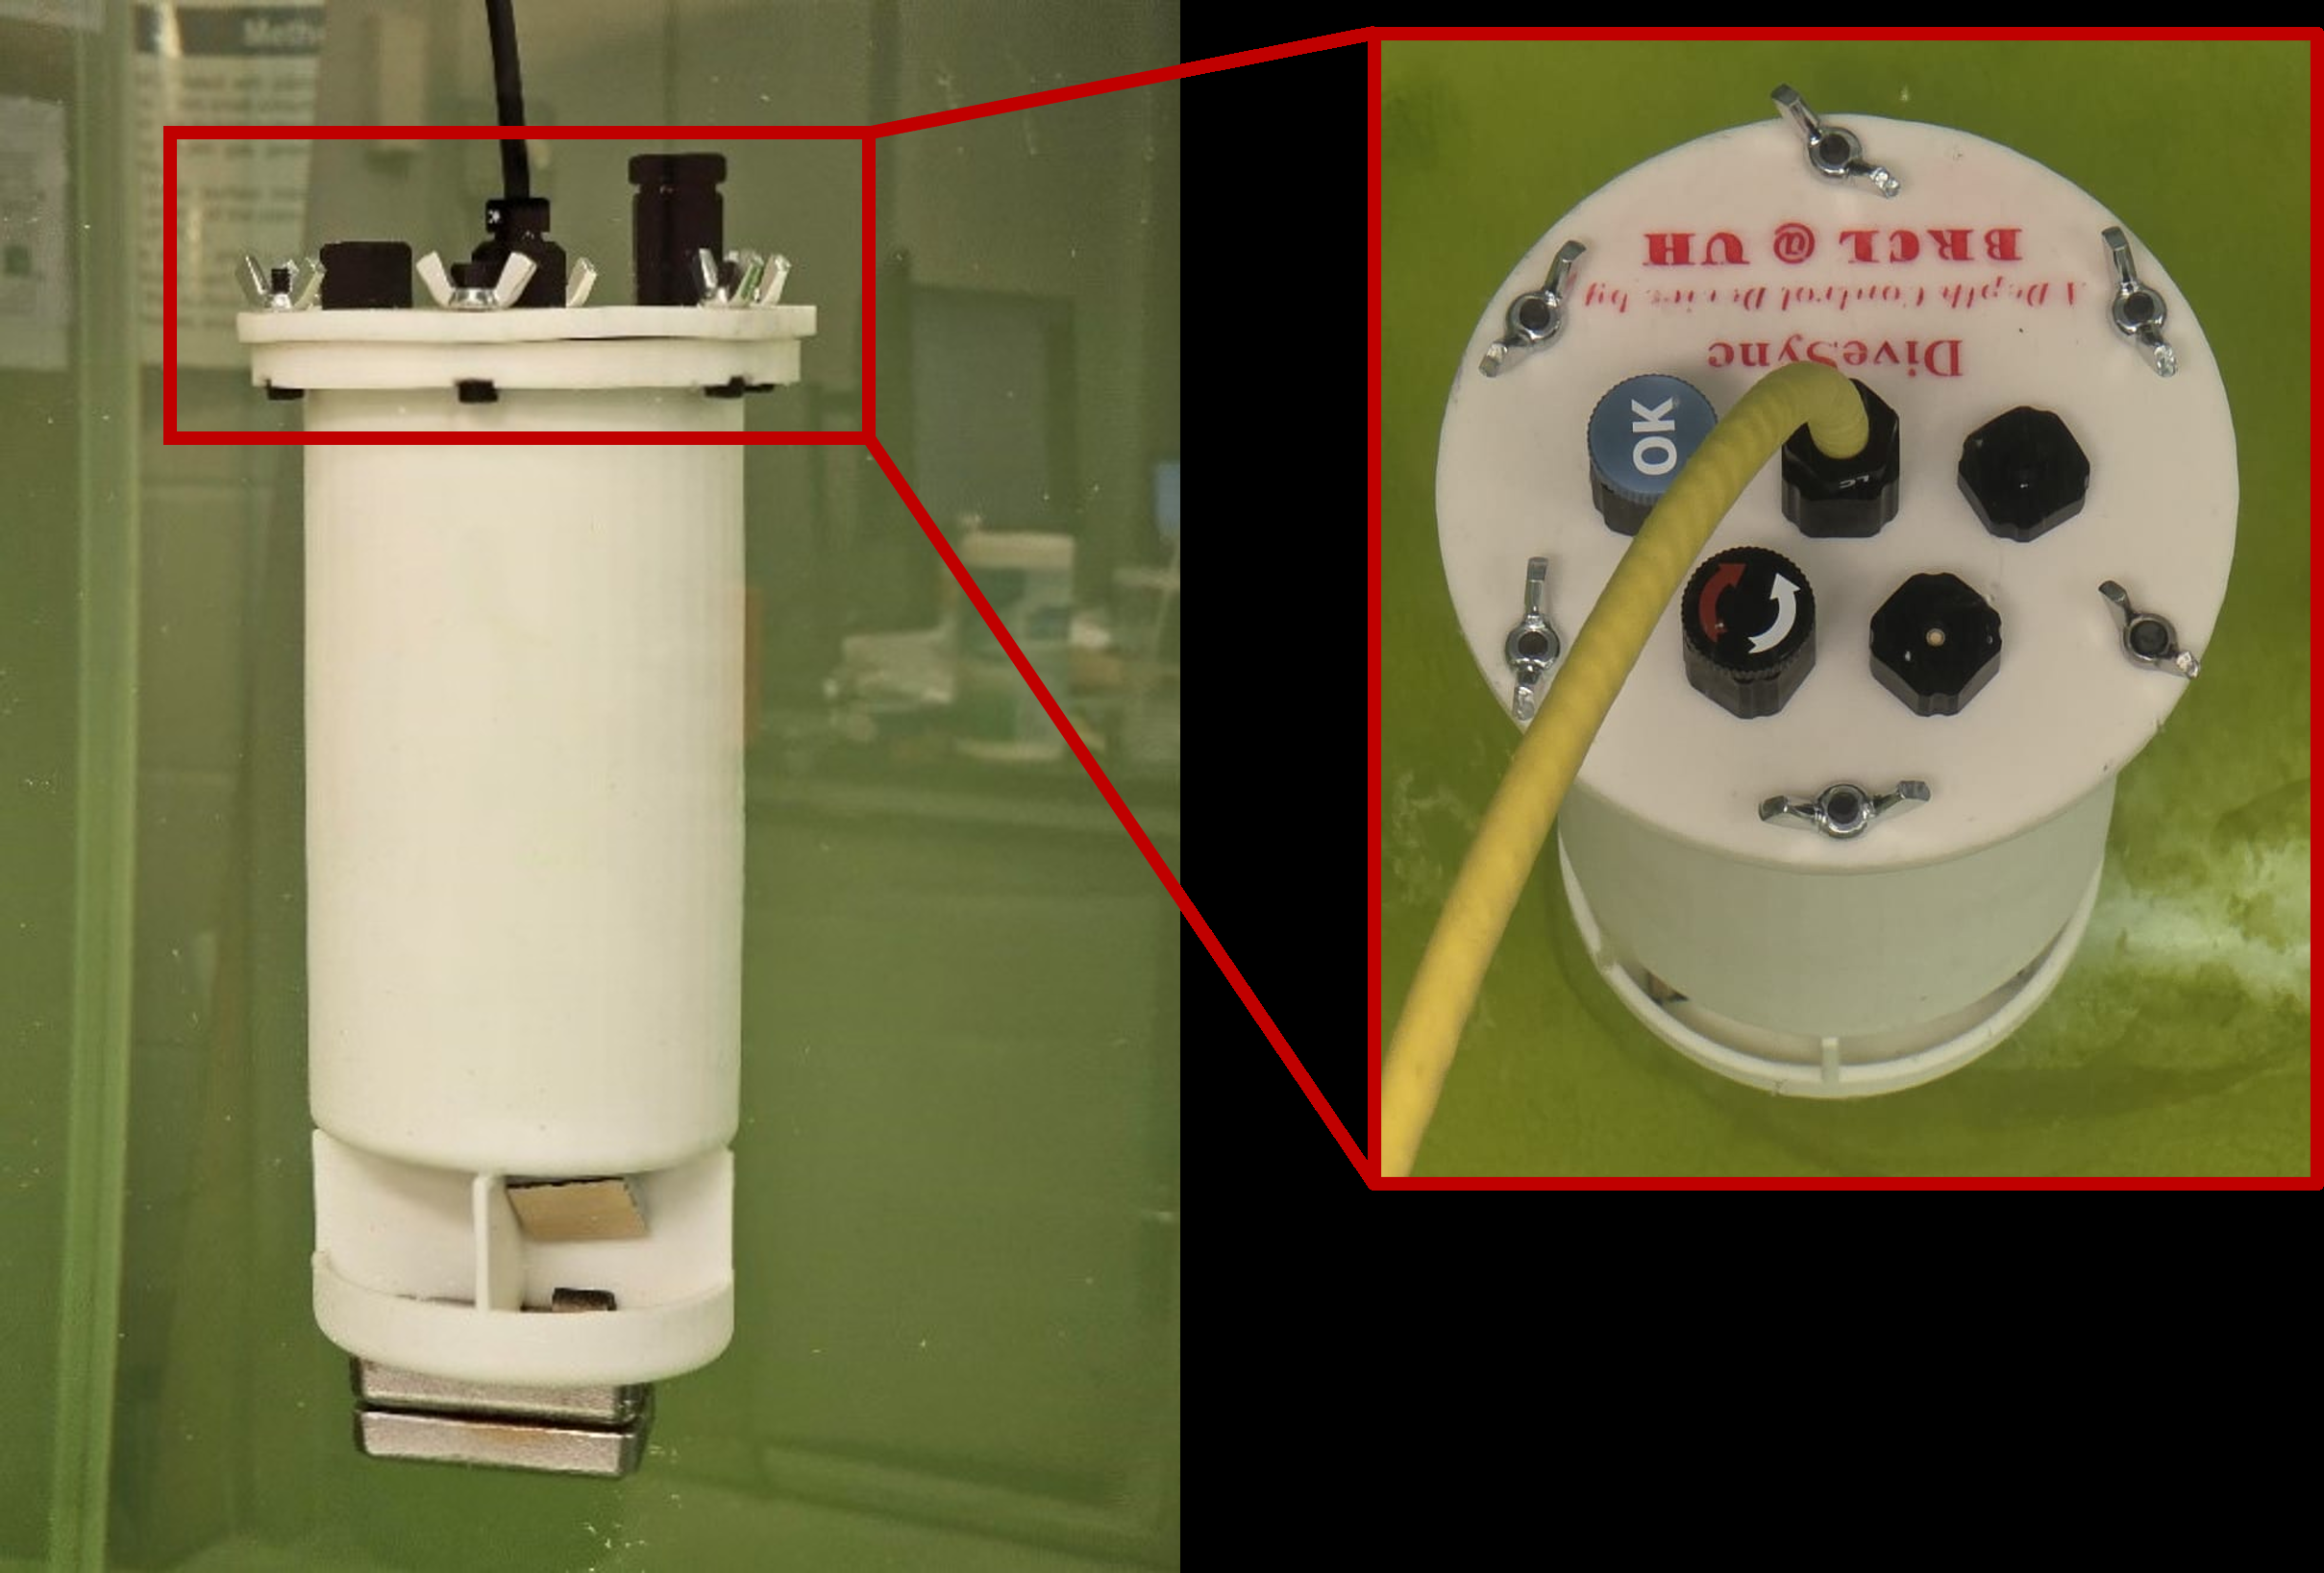
\includegraphics[width=0.72\textwidth]{Fig/ch2_bcd_fabricated.png}
    \caption{Fabricated standalone BCD for depth-control experiments.}
    \label{fig:ch2_bcd_fabricated}
\end{figure}

The AquaNavigator body parts were fabricated using resin-based additive manufacturing and assembled around the propulsion, steering, enclosure, and sensing modules. The fabricated robot is shown in Fig.~\ref{fig:ch2_aquanavigator_real}. The platform is used as a laboratory and pool-scale research system for studying underwater propulsion, buoyancy control, perception, and environmental sensing in controlled water environments.

\begin{figure}[t]
    \centering
    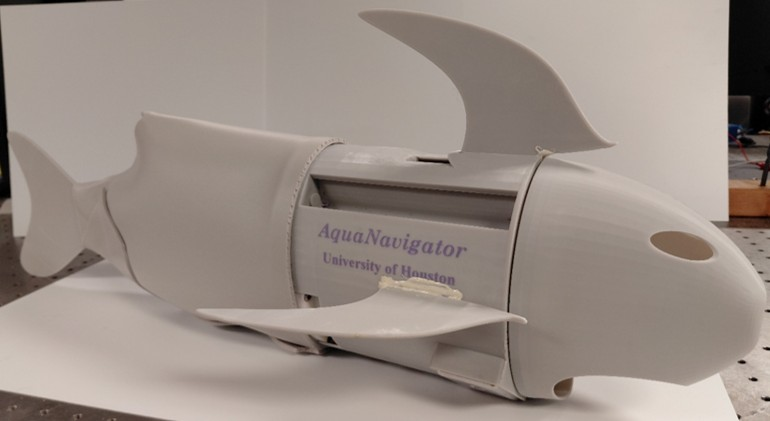
\includegraphics[width=0.7\textwidth]{Fig/ch2_aquanavigator_real.jpg}
    \caption{Fabricated AquaNavigator robotic fish experimental platform.}
    \label{fig:ch2_aquanavigator_real}
\end{figure}

With the BCD and AquaNavigator fabricated, the next step is to validate the buoyancy model and design controllers that respect the practical limits of the actuator and device.

\chapter{Model Validation and Control Design}

Chapter~2 developed the physical design and dynamic models of the standalone buoyancy control device and AquaNavigator. This chapter uses those models for validation and control design. The chapter has two connected control themes. The first is depth regulation of the BCD, where the main issues are unstable neutral buoyancy, piston stroke limits, actuator voltage limits, and mismatch between the model and the fabricated hardware. The second is planar pipeline tracking of AquaNavigator, where the robot is controlled by redirecting tail-generated thrust using camera feedback.

The chapter is organized in the same order as the control development. First, the BCD model is validated using open-loop actuator and depth measurements. Second, a constrained model predictive controller is described for BCD depth regulation. Third, an extremum seeking control approach is presented as a later constraint-aware alternative that adapts controller gains online. Fourth, the pipeline-tracking controller for AquaNavigator is introduced. Fifth, the robotic-fish simulator is summarized because it is used to evaluate visual-servo control before pool experiments. The final sections collect the results and close the chapter.

\section{Model Validation of the BCD}

The BCD model in Chapter~2 couples vertical motion with piston-actuator dynamics. Before using that model for controller design, its dominant behavior must be checked against hardware measurements. The validation procedure uses an open-loop experiment with the standalone BCD \cite{Masood2026ESCBCD}. The goal is not to prove that the model captures every nonlinear effect. Instead, the goal is to verify that the model reproduces the main actuator response and the resulting depth response well enough to support controller design and to identify where unmodeled effects remain.

The validation experiment is performed on the standalone BCD, also referred to as DiveSync. The actuator has built-in self-locking up to approximately $50$~N of holding force. For the tested depth range, the hydrostatic load is below this threshold, so the actuator can be treated as holding its position when it is not actively driven. This makes an open-loop validation meaningful over the tested operating range.

In the experiment, a square-wave voltage input $u(t)$ is applied to the linear actuator. The actuator position $z_a(t)$ and the device depth $z_d(t)$ are recorded simultaneously. The same input is then applied to the model, and the simulated actuator and depth responses are compared with the measured responses. The comparison is later shown in the results section. This validation method is useful because it separates two parts of the model: the actuator subsystem is checked through $z_a(t)$, while the buoyancy/depth subsystem is checked through $z_d(t)$.

\section{MPC-Based BCD Control Design}

The first closed-loop BCD controller considered in this dissertation is a constrained model predictive controller (MPC) \cite{Masood2023MPCBCD}. MPC is appropriate for the BCD because actuator motion is physically bounded. If a controller commands piston motion beyond the available stroke, the device cannot produce the requested buoyancy change. Near neutral buoyancy, this loss of control authority can cause persistent drift or unstable depth behavior. The MPC formulation addresses this by optimizing depth tracking while explicitly respecting the piston-position constraint.

The MPC objective is written as a finite-horizon quadratic cost,
\begin{equation}
    J(t_0) =
    \sum_{t=t_0}^{t_0+T}
    \left[
        \left(C\mathbf{x}(t)-r(t)\right)^T
        Q
        \left(C\mathbf{x}(t)-r(t)\right)
        +
        \mathbf{u}(t)^T R \mathbf{u}(t)
    \right],
    \label{eq:ch3_mpc_cost}
\end{equation}
where $\mathbf{x}$ is the model state, $C\mathbf{x}$ is the predicted depth output, $r$ is the reference depth, $Q$ penalizes tracking error, and $R$ penalizes control effort. The controller is subject to the hard actuator bound
\begin{equation}
    |u| \leq u_b ,
    \label{eq:ch3_mpc_constraint}
\end{equation}
where $u_b$ is the maximum admissible piston command. For the BCD experiments, the bound is $u_b=20$~mm. After the constrained optimization is solved, the first control move is applied and the horizon is shifted forward.

For the implemented controller, the plant is discretized with a sampling time of $0.1$~s. The prediction horizon is $80$ steps, the control horizon is $20$ steps, and the weights are set to $Q=1$ and $R=40$. Only the depth state is directly measured by the depth sensor. The remaining states are estimated by the internal observer in the MPC implementation, so the controller can use full-state feedback in the optimization. The control structure is shown in Fig.~\ref{fig:ch3_mpc_control_scheme}.

\begin{figure}[t]
    \centering
    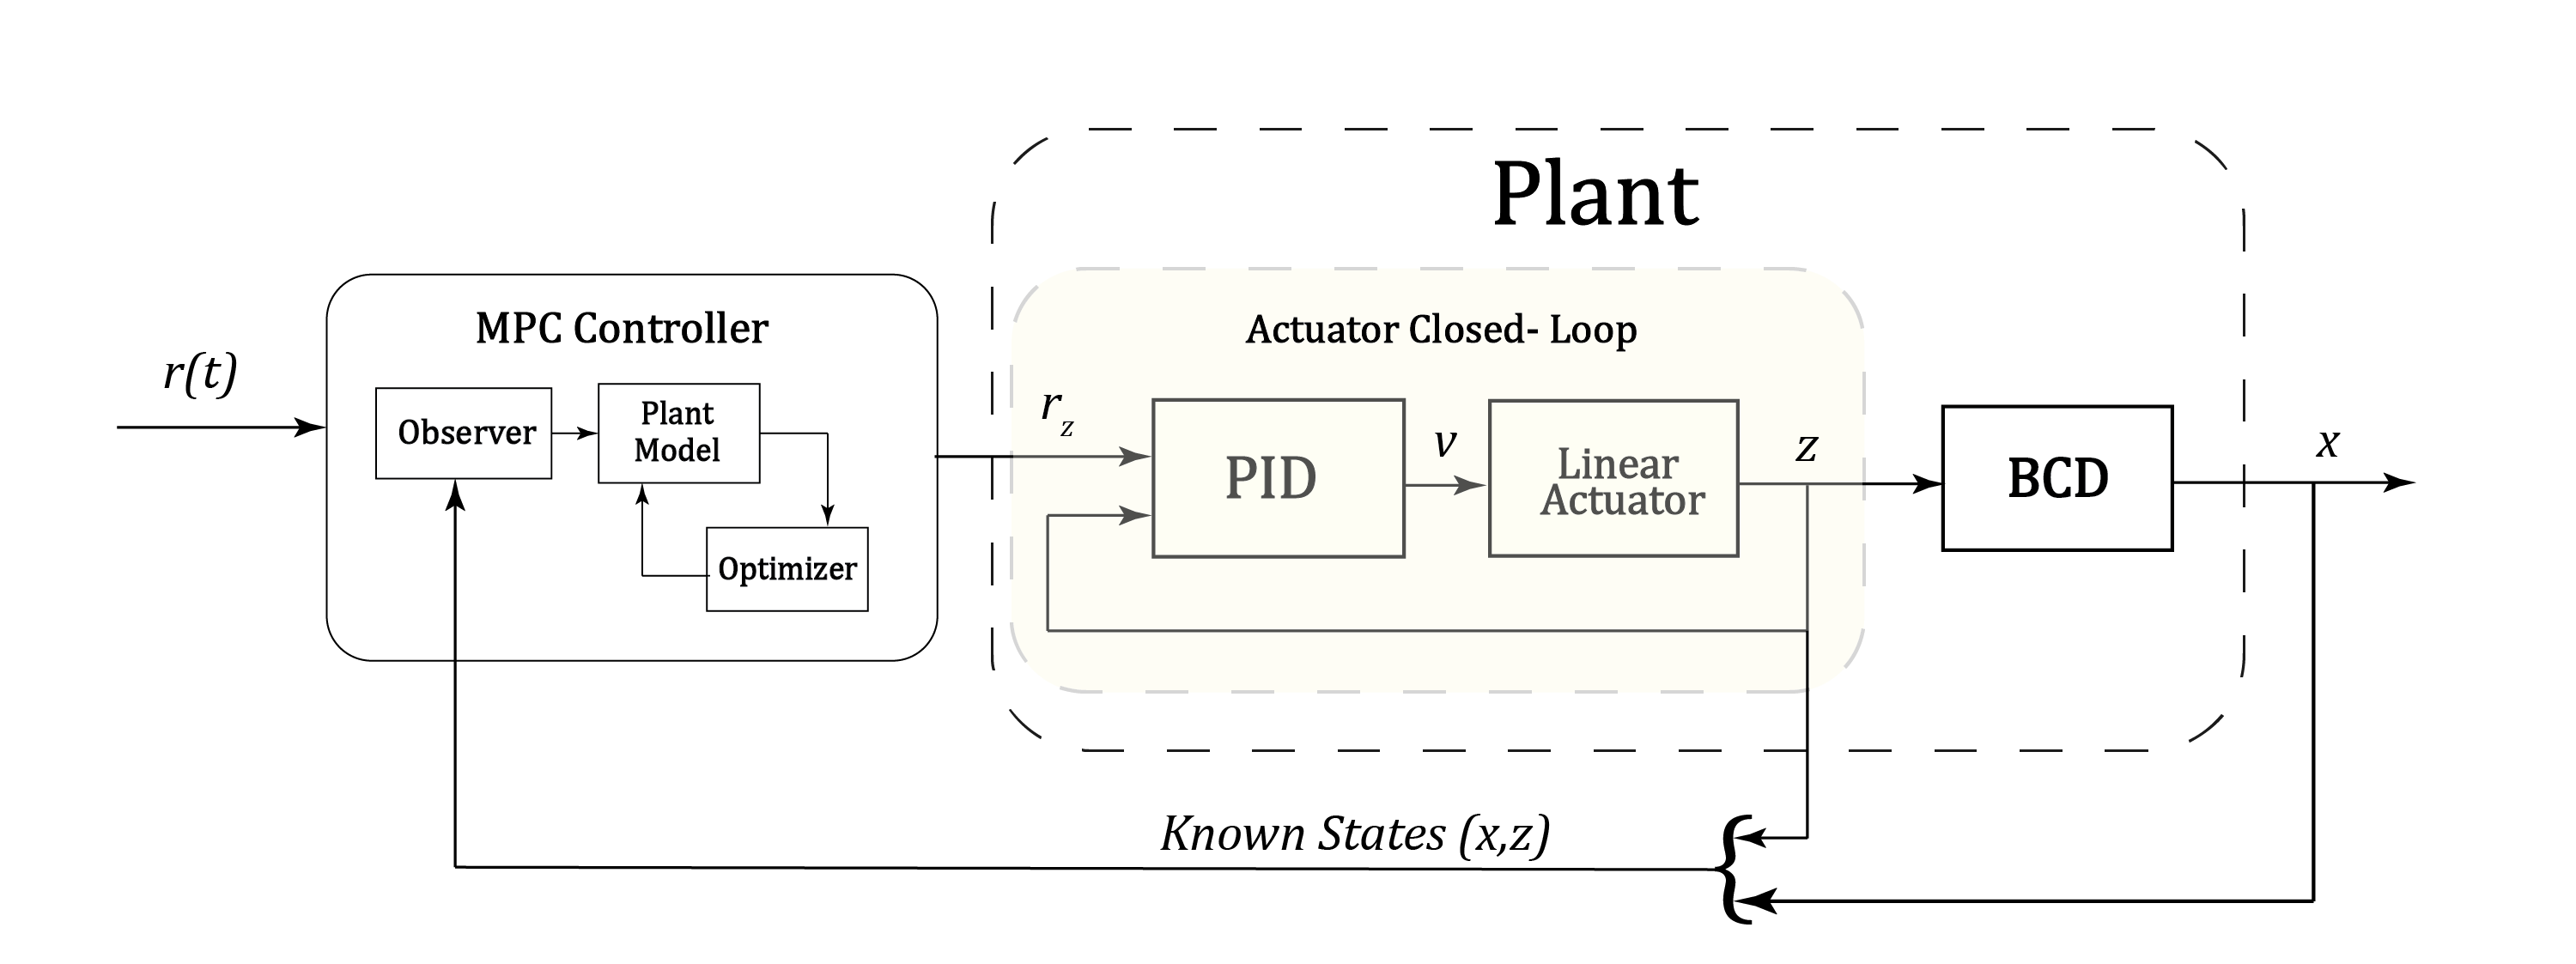
\includegraphics[width=0.82\textwidth]{Fig/ch3_mpc_control_scheme.png}
    \caption{MPC control structure for the BCD.}
    \label{fig:ch3_mpc_control_scheme}
\end{figure}

\begin{table}[t]
    \centering
    \caption{MPC simulation and experiment design parameters.}
    \label{tab:ch3_mpc_parameters}
    \begin{tabular}{lll}
        \hline
        Parameter & Value & Unit \\
        \hline
        Sampling time & 0.1 & s \\
        Prediction horizon & 80 & steps \\
        Control horizon & 20 & steps \\
        Actuator bound & 20 & mm \\
        Output-error weight $Q$ & 1 & -- \\
        Input-effort weight $R$ & 40 & -- \\
        Damping coefficient & 0.192 & N s/m \\
        Device mass & 0.683 & kg \\
        \hline
    \end{tabular}
\end{table}

\section{Extremum Seeking Control of the BCD}

The MPC design explicitly handles constraints, but its performance depends on the accuracy of the plant model. The fabricated BCD includes actuator dead zone, backlash, friction, direction-dependent behavior, pressure loading, sensor noise, and disturbances from cable tension and tank-wall effects. These effects are difficult to capture exactly in a fixed model. The ESC-based BCD controller therefore uses extremum seeking control (ESC) as an online adaptation layer for depth regulation \cite{Masood2026ESCBCD}.

The BCD has four main dynamic states: depth, depth velocity, piston position, and piston velocity. Depth and piston position are measured directly, while the velocity states are estimated. The control input is actuator voltage, and both voltage and piston stroke are bounded. A depth-only PID controller is not sufficient for this system because it can reduce depth error while unknowingly driving the piston toward a stroke limit. The ESC design therefore treats controller tuning as an online optimization problem shaped by physical constraints.

Classical ESC can be understood locally by considering an unknown static map $y=f(\theta)$ near an extremum $\theta^\ast$:
\begin{equation}
    f(\theta)
    \approx
    f(\theta^\ast)
    + \frac{1}{2}f''(\theta^\ast)(\theta-\theta^\ast)^2 .
    \label{eq:ch3_esc_static_map}
\end{equation}
A sinusoidal perturbation is added to the decision variable, and the measured response is high-pass filtered, demodulated, low-pass filtered, and integrated to update the estimate of the improving parameter. The BCD does not satisfy the ideal static-map setting exactly because the depth response is dynamic and trajectory-dependent. For that reason, three ESC structures were considered.

The first structure applies ESC directly to the actuator voltage. This is useful as a baseline, but voltage does not directly determine depth; it first changes piston motion, and the unstable depth dynamics then evolve from the resulting buoyancy change. The second structure adds an inner actuator-position loop. This improves actuator behavior, but it still does not stabilize the depth state by itself. The third structure is the one used for the main ESC results: an ESC-tuned PD depth controller. Its inner depth-control law is
\begin{equation}
    u = K_p(r-z) - K_d \dot{z},
    \label{eq:ch3_esc_pd_law}
\end{equation}
where $r$ is the depth reference, $z$ is measured depth, and $\dot{z}$ is estimated depth velocity. The ESC layer adjusts the effective gains online instead of fixing them manually. The proposed architecture is shown in Fig.~\ref{fig:ch3_esc_tuned_pd_scheme}.

\begin{figure}[t]
    \centering
    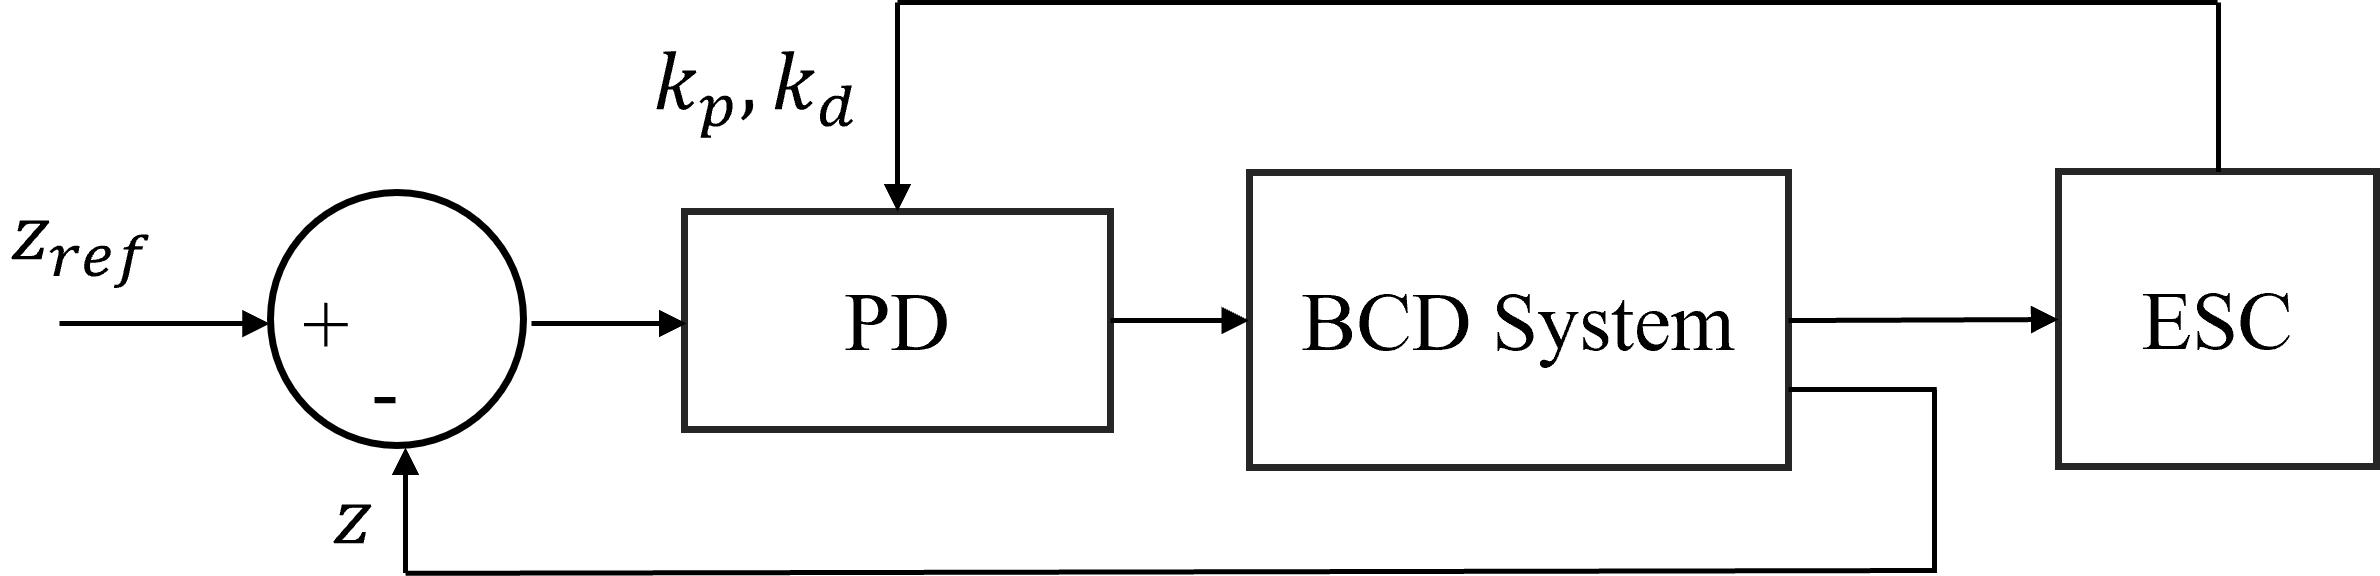
\includegraphics[width=0.84\textwidth]{Fig/ch3_esc_tuned_pd_scheme.png}
    \caption{ESC-tuned PD controller architecture for BCD.}
    \label{fig:ch3_esc_tuned_pd_scheme}
\end{figure}

Two cost functions are important. The first penalizes actuator motion:
\begin{equation}
    J = \dot{x}^2 ,
    \label{eq:ch3_esc_velocity_cost}
\end{equation}
where $x$ is piston displacement. This encourages reduced actuator activity, but it does not directly distinguish useful piston motion from unsafe piston motion near the stroke limits. The second cost adds a deadzone penalty around the neutral piston position:
\begin{equation}
    J_z =
    w_z
    \left[
        \max\left(0,\left|z_a-z_{a,\mathrm{eq}}\right|-\delta_z\right)
    \right]^2 ,
    \label{eq:ch3_esc_deadzone_cost}
\end{equation}
where $z_a$ is piston position, $z_{a,\mathrm{eq}}$ is the neutral piston position, $\delta_z$ is the safe-band half-width, and $w_z$ is the penalty weight. When the piston remains inside the safe band, this penalty is zero. When it moves toward a stroke limit, the penalty activates and drives adaptation toward gains that pull the piston back toward the middle of the stroke.

For the hardware experiment, the cost combines depth tracking with the deadzone penalty and a piston-velocity term:
\begin{equation}
    J =
    (r-\hat{z})^2
    +
    w_z
    \left[
        \max\left(0,\left|z_a-z_{a,\mathrm{eq}}\right|-\delta_z\right)
    \right]^2
    +
    w_{\dot{z}}\dot{z}_a^2 .
    \label{eq:ch3_esc_experimental_cost}
\end{equation}
The first term improves depth tracking, the second term protects the piston stroke margin, and the third term discourages unnecessary actuator motion. In the implemented experiment, the derivative gain is tied to the proportional gain by $K_d=T_DK_p$, so one ESC channel adapts $\hat{K}_p$ and the derivative gain follows through the fixed time constant $T_D$.

\begin{table}[t]
    \centering
    \caption{ESC-tuned PD experimental parameter value summary.}
    \label{tab:ch3_esc_parameters}
    \begin{tabular}{lll}
        \hline
        Parameter & Symbol & Value \\
        \hline
        Derivative time constant & $T_D$ & 10.0 s \\
        Initial proportional gain & $K_{p,0}$ & 15.0 \\
        Gain lower bound & $K_{p,\min}$ & 1.0 \\
        Gain upper bound & $K_{p,\max}$ & 35.0 \\
        ESC integration gain & $\gamma$ & 5000.0 \\
        Dither frequency & $\omega_{\mathrm{ESC}}$ & $\pi$ rad/s \\
        Dither amplitude & $a$ & 1.0 \\
        Demodulation gain & $b$ & 2.0 \\
        Piston deadzone weight & $w_z$ & 2.0 \\
        Piston deadzone half-width & $\delta_z$ & 15 mm \\
        Piston equilibrium & $z_{a,\mathrm{eq}}$ & 25 mm \\
        Piston stroke limits & $[z_{a,\min},z_{a,\max}]$ & $[0,50]$ mm \\
        Voltage limits & $[u_{\min},u_{\max}]$ & $[-12,+12]$ V \\
        ESC update period & $\Delta t_{\mathrm{ESC}}$ & 50 ms \\
        \hline
    \end{tabular}
\end{table}

\section{Pipeline Tracking Control of AquaNavigator}

The pipeline-tracking controller uses AquaNavigator as a camera-guided planar swimming robot \cite{Masood2025Pipeline}. In this chapter, pipeline tracking is treated as a control-design problem for the robotic fish. The sensing and inspection interpretation is developed later in the infrastructure-monitoring chapter. The control objective is to align the fish with a pipeline-like feature detected in the camera image and reduce the lateral image-space error. Depth control is not active in these pipeline-tracking experiments.

The onboard camera is mounted near the front of the robot and tilted downward. The image stream is sent to a host computer where OpenCV-based processing converts the frame to grayscale, applies edge detection, and uses a Hough-transform pipeline to identify the dominant line corresponding to the pipeline. The detected pipeline is represented as an image-space vector $\vec{P}$. The robot heading is represented by a heading vector $\vec{h}$ fixed in the image frame because the camera is fixed relative to the robot body. The tracking error is an angle $\psi_e$ formed from these vectors. The controller drives $\psi_e$ toward zero so the robot becomes aligned with the detected pipeline.

The visual-servoing control structure is shown in Fig.~\ref{fig:ch3_pipeline_control_scheme}. The controller uses a PID law to command the tail-bias angle:
\begin{equation}
    \delta(i+1)
    =
    K_p\psi_e(i)
    +
    K_i\sum_{j=i-w_i}^{i}\psi_e(j)\Delta t
    +
    K_d\frac{\psi_e(i)-\psi_e(i-1)}{\Delta t}.
    \label{eq:ch3_pipeline_pid}
\end{equation}
The tail-beat frequency is held constant during the tracking experiment, while $\delta$ changes the direction of the average tail-generated thrust. The commanded tail-bias angle is saturated at $\pm 20^\circ$ in the embedded safety logic. This saturation corresponds to the practical turning limit of the prototype; experiments with the saturated command indicated a turning radius of approximately $3$~m.

\begin{figure}[t]
    \centering
    \includegraphics[width=0.82\textwidth]{Fig/ch3_pipeline_control_scheme.png}
    \caption{Pipeline-tracking visual servoing control scheme overview.}
    \label{fig:ch3_pipeline_control_scheme}
\end{figure}

\begin{figure}[t]
    \centering
    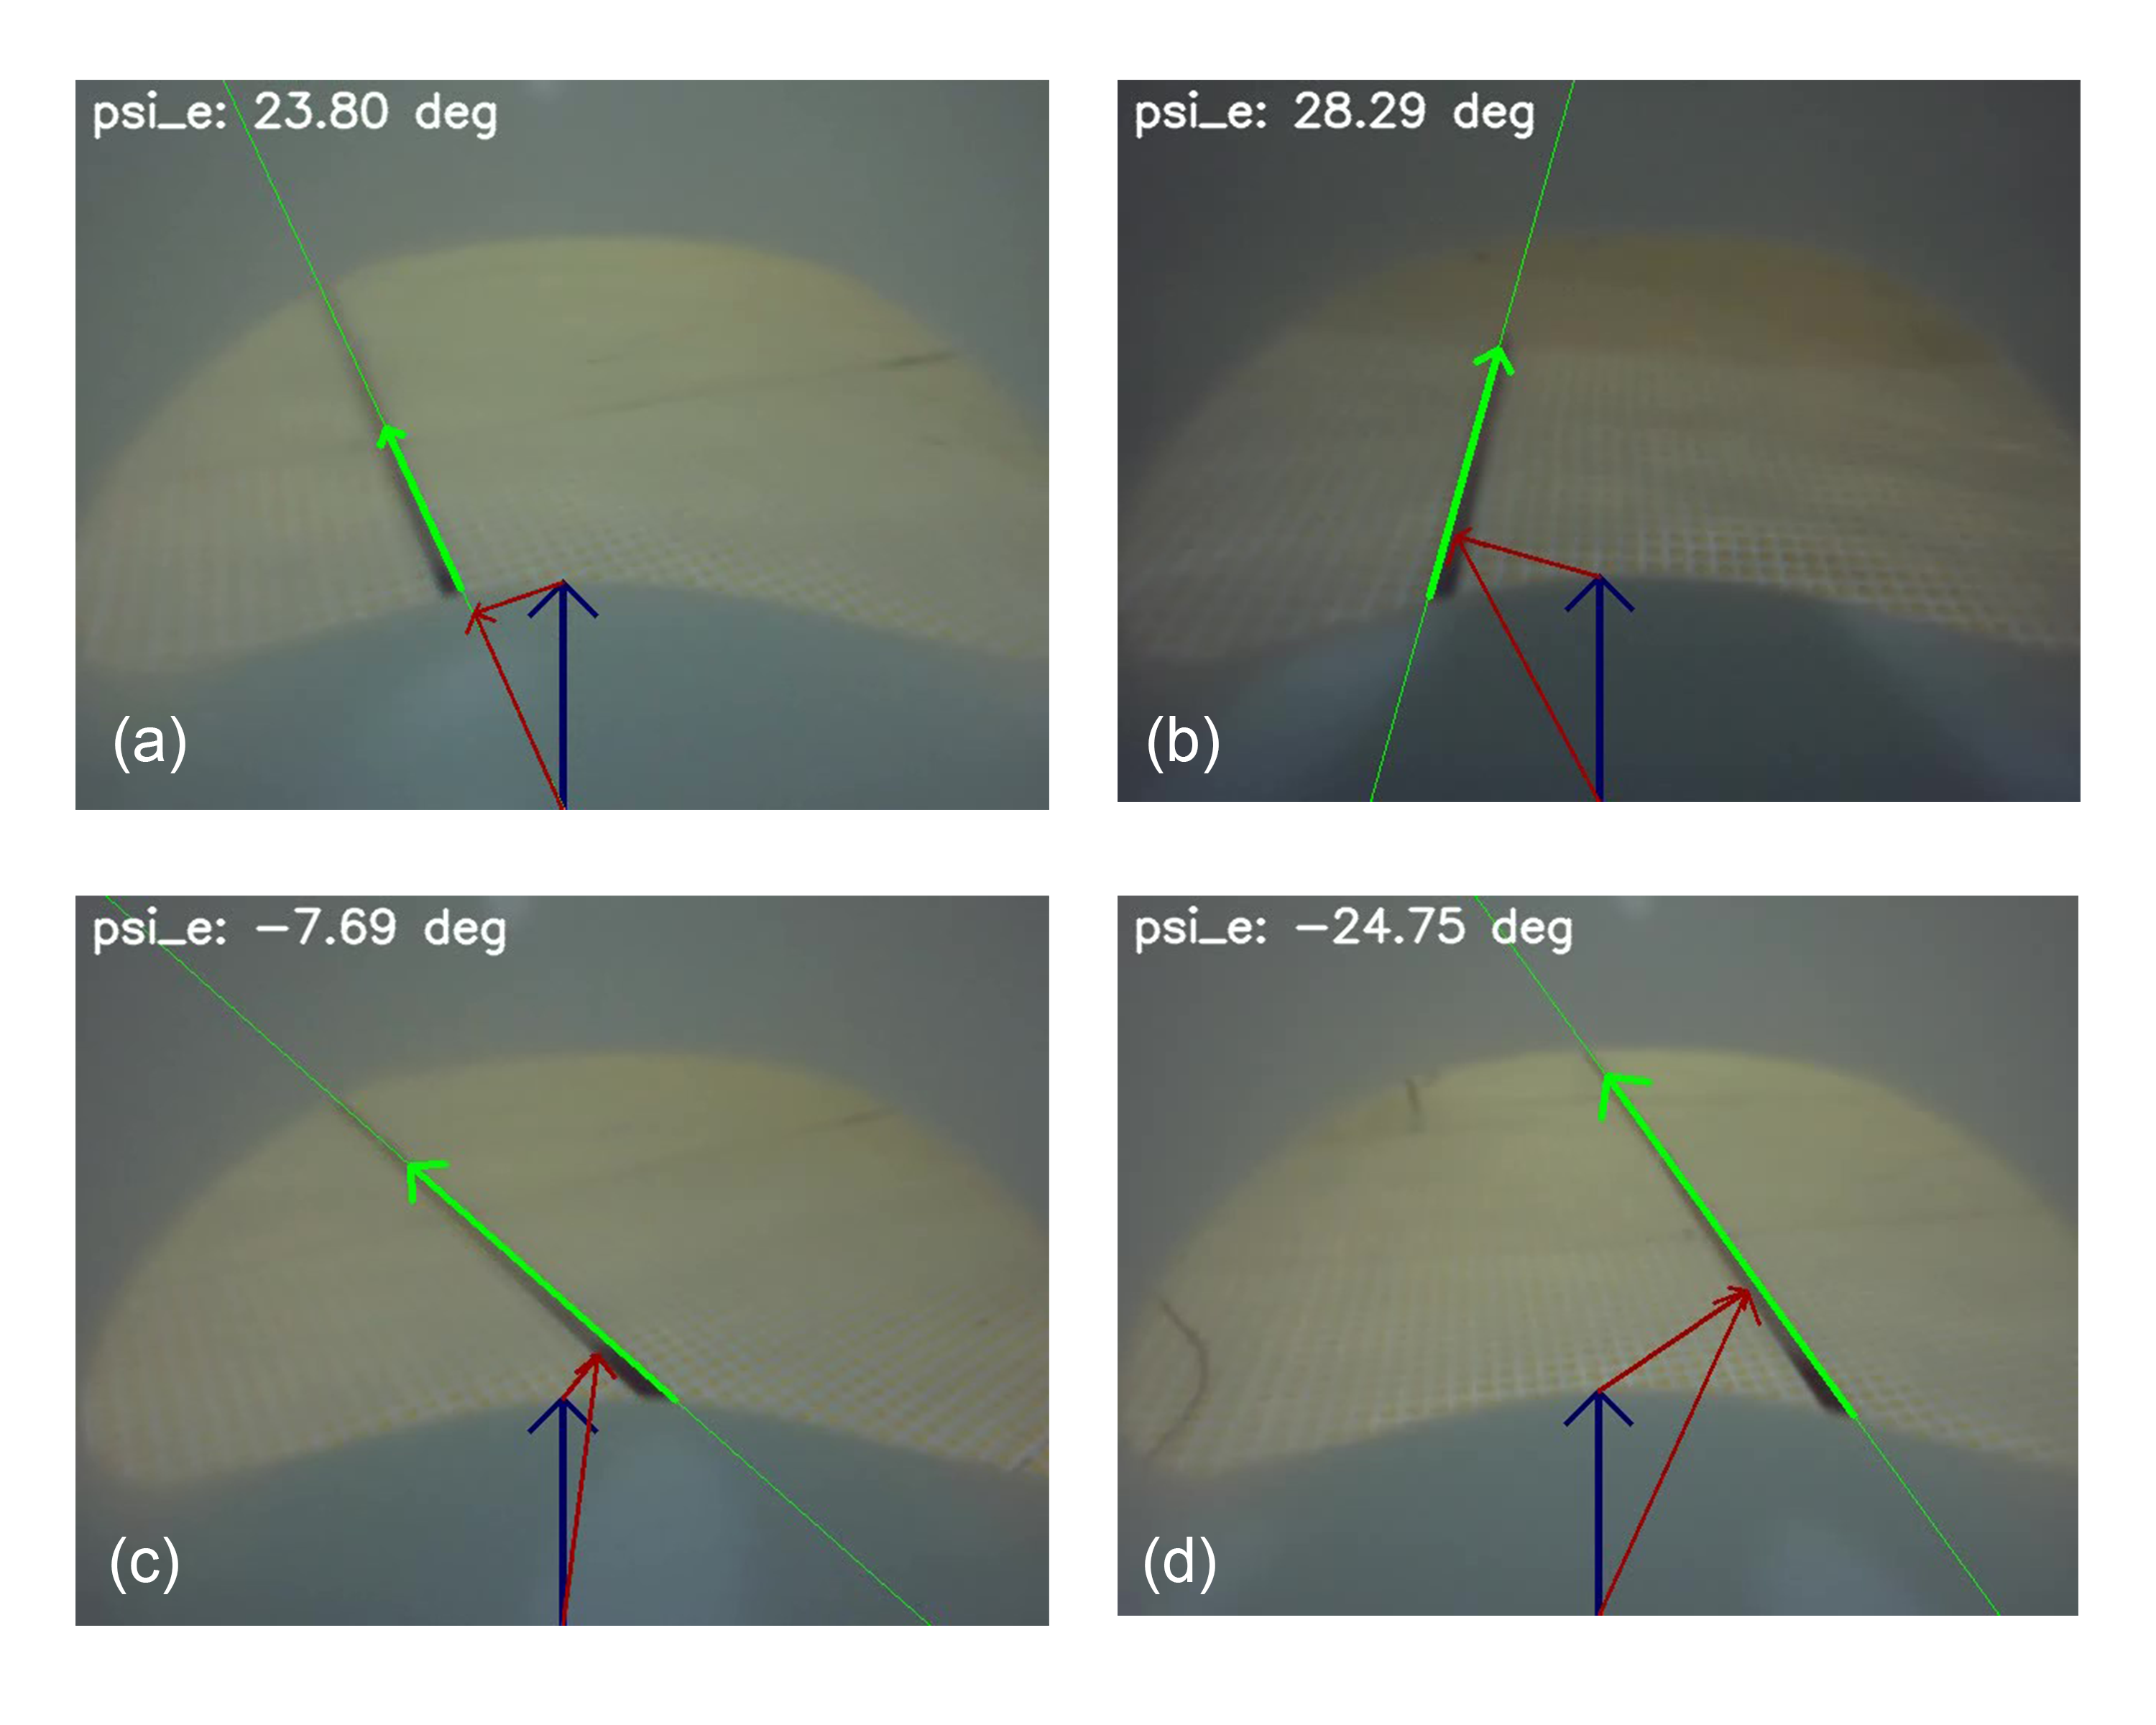
\includegraphics[width=0.82\textwidth]{Fig/ch3_pipeline_camera_vectors.png}
    \caption{Camera pipeline vectors for visual servoing control.}
    \label{fig:ch3_pipeline_camera_vectors}
\end{figure}

\section{Robotic Fish Simulator}

The simulator is used to test the robotic-fish model and visual-servo control before pool experiments. It numerically integrates the planar dynamic model from Chapter~2 using a fixed time step and represents the water tank, pipeline, and robotic fish as modular components. The simulator stores state and control histories so that controller gains, tracking errors, and trajectory behavior can be evaluated before operating the physical robot.

For the pipeline-tracking experiment, the simulated tank is $10$~m long and $5$~m wide, with a pipeline placed on the bottom surface. The robot is initialized $0.5$~m away from the pipeline, and the tail-beat frequency is set to $11$~rad/s. The simulation is run for $35$~s with a time step of $0.05$~s. Because tail-driven propulsion produces head and body oscillation, the raw image-space tracking angle contains high-frequency motion. A moving-average filter with a $15$-sample window is applied to $\psi_e$. At a sampling frequency of $20$~Hz, this corresponds to a smoothing window of $0.75$~s and an approximate cutoff frequency of $0.67$~Hz.

Both position-based visual servoing (PBVS) and image-based visual servoing (IBVS) are tested in the simulator. PBVS uses world-frame position and orientation information, which is available in simulation but not directly available on the physical robotic fish. IBVS uses image-space quantities, which better matches the physical experiment because the robot relies on its onboard camera rather than an underwater global localization system. For this reason, IBVS is the preferred implementation for the pool experiment.

\section{Results and Discussion}

\subsection{BCD Open-Loop Model Validation}

The open-loop validation result is shown in Fig.~\ref{fig:ch3_bcd_open_loop_validation}. The actuator position predicted by the model follows the measured actuator response with an RMSE of $1.96$~mm. This confirms that the identified actuator time constant and gain capture the main piston motion over the tested range. The depth response has an RMSE of $23.07$~mm. The model reproduces the qualitative oscillatory behavior of the device, but the remaining error indicates that tank-wall effects, depth-dependent drag variation, and neutral-buoyancy offsets are not fully captured.

\begin{figure}[t]
    \centering
    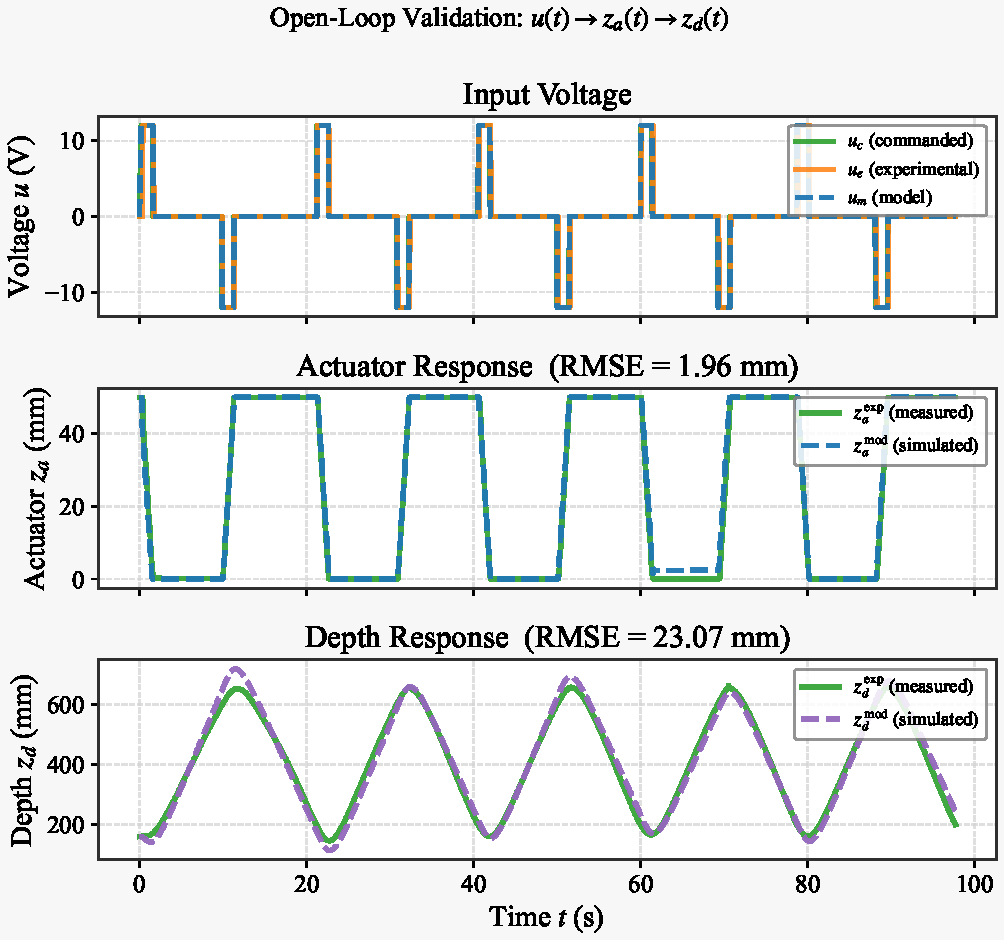
\includegraphics[width=0.88\textwidth]{Fig/ch3_bcd_open_loop_validation.pdf}
    \caption{Open-loop BCD validation with model comparison.}
    \label{fig:ch3_bcd_open_loop_validation}
\end{figure}

The validation result supports using the model for controller design, but it also motivates the ESC controller used later in this chapter. MPC can exploit the identified model and constraints, but unmodeled actuator nonlinearities and environmental effects remain important in hardware.

\subsection{MPC Depth-Control Results}

Figure~\ref{fig:ch3_mpc_simulation} shows the MPC simulation response for the selected $Q=1$, $R=40$ tuning. The relatively large input penalty causes the controller to trade response speed for reduced control effort. This is appropriate for an actuator-limited buoyancy device because unnecessarily aggressive piston commands can push the system toward saturation.

\begin{figure}[t]
    \centering
    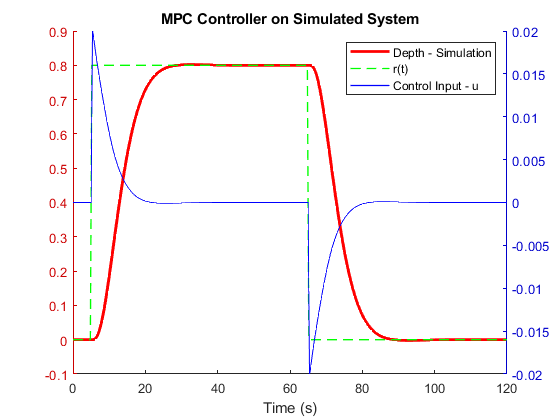
\includegraphics[width=0.62\textwidth]{Fig/ch3_mpc_simulation.png}
    \caption{MPC simulation response for BCD depth tracking.}
    \label{fig:ch3_mpc_simulation}
\end{figure}

\begin{figure}[t]
    \centering
    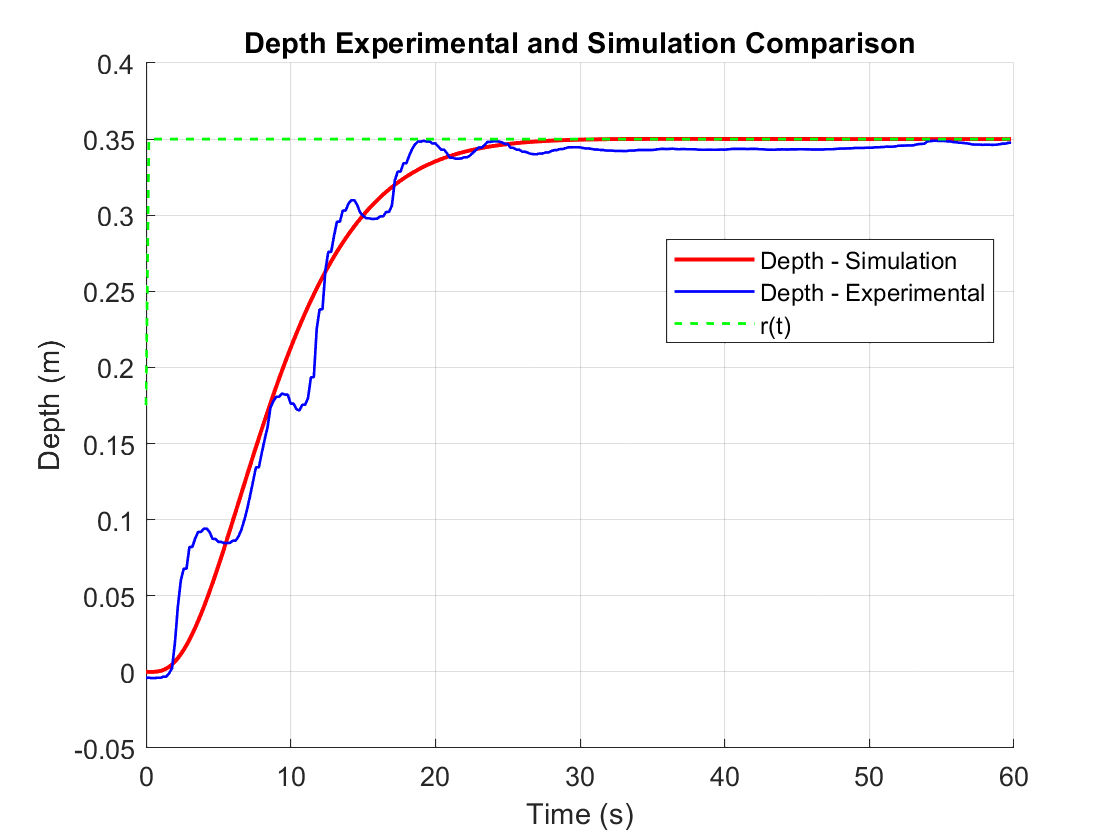
\includegraphics[width=0.68\textwidth]{Fig/ch3_mpc_experiment.png}
    \caption{Experimental MPC response compared with simulation.}
    \label{fig:ch3_mpc_experiment}
\end{figure}

The experimental MPC result is shown in Fig.~\ref{fig:ch3_mpc_experiment}. The experiment is performed with a $35$~mm step command and compared against the simulated plant output. The response shows acceptable steady-state behavior, while the transient contains vibration and mismatch that are attributed to nonlinear physical effects not included in the simplified model. The MPC experiment reported steady-state tracking within approximately two percent error bounds \cite{Masood2023MPCBCD}.

\subsection{ESC Depth-Control Results}

Before the depth-loop ESC experiments, the actuator loop is checked independently. Figure~\ref{fig:ch3_bcd_actuator_loop_result} shows representative actuator-position tracking, command activity, and depth telemetry. The position loop tracks commanded setpoints while reducing measurement jitter using median filtering and an $\alpha$-$\beta$ estimator. This actuator-loop behavior is important because the ESC experiments assume that piston-position commands can be executed repeatably enough for outer-loop adaptation.

\begin{figure}[t]
    \centering
    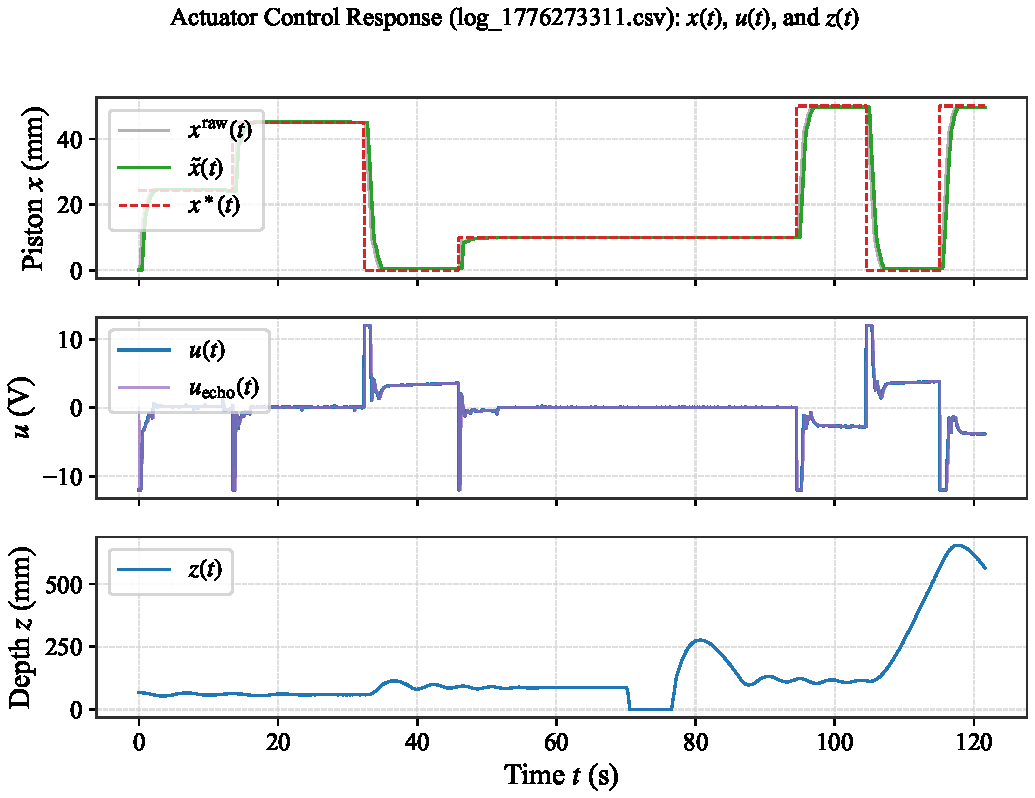
\includegraphics[width=0.6\textwidth]{Fig/ch3_bcd_actuator_loop_result.pdf}
    \caption{Actuator-loop validation before ESC depth experiments.}
    \label{fig:ch3_bcd_actuator_loop_result}
\end{figure}

The ESC-tuned PD controller is evaluated first in simulation with a reference that switches from sinusoidal depth motion to square-wave depth commands. Figure~\ref{fig:ch3_esc_velocity_penalty_sim} shows the velocity-penalty objective. Depth tracking is maintained, the voltage remains within $\pm 12$~V, and the piston remains within its stroke limits. However, because the cost penalizes actuator velocity rather than proximity to stroke limits, the piston can approach the bounds during aggressive square-wave transients.

\begin{figure}[t]
    \centering
    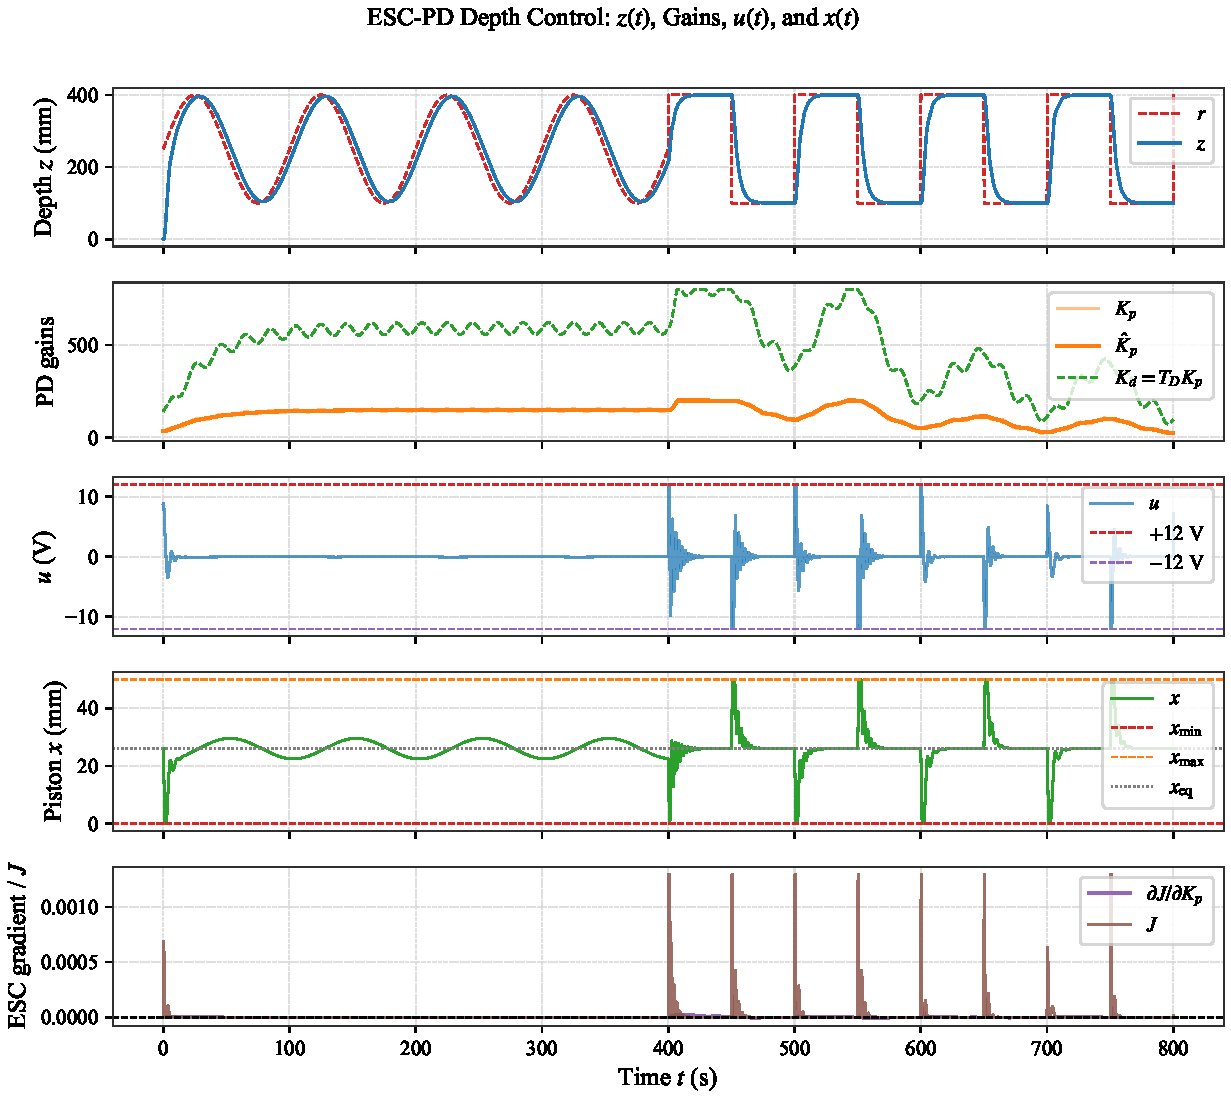
\includegraphics[width=0.65\textwidth]{Fig/ch3_esc_velocity_penalty_sim.pdf}
    \caption{ESC simulation with velocity-penalty objective function.}
    \label{fig:ch3_esc_velocity_penalty_sim}
\end{figure}

Figure~\ref{fig:ch3_esc_deadzone_penalty_sim} shows the simulation with the deadzone piston-position penalty. With $w_z=2.0$ and $\delta_z=15$~mm, the piston remains more tightly confined around the neutral stroke. The key difference is that adaptation is activated directly by stroke-margin violation rather than by general actuator motion. This makes the cost more aligned with the safety requirement of a hard-bound actuator.

\begin{figure}[t]
    \centering
    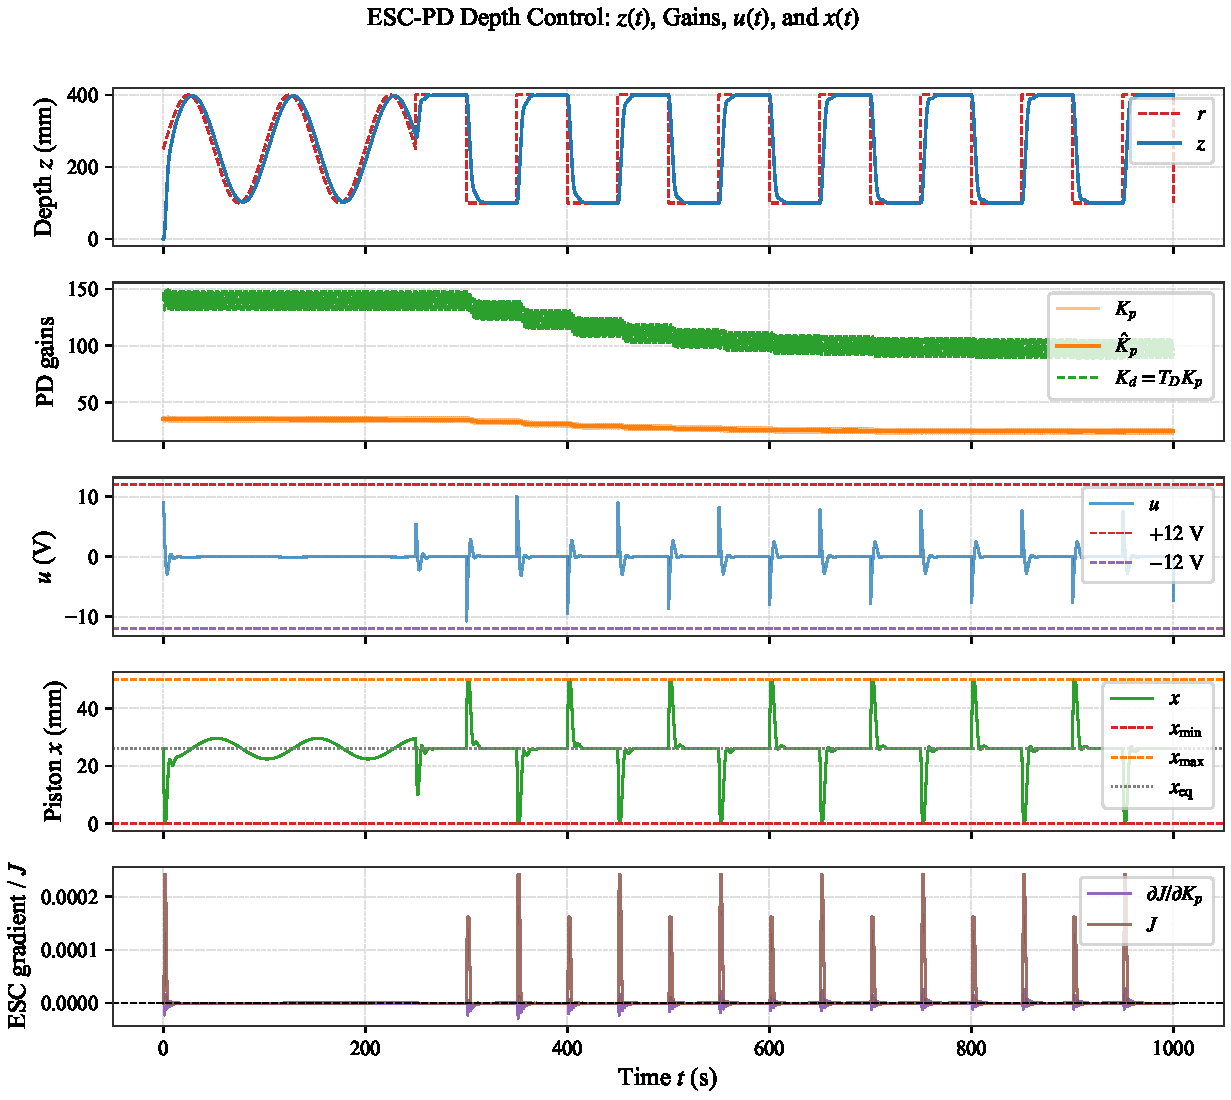
\includegraphics[width=0.65\textwidth]{Fig/ch3_esc_deadzone_penalty_sim.pdf}
    \caption{ESC simulation with deadzone piston-position penalty.}
    \label{fig:ch3_esc_deadzone_penalty_sim}
\end{figure}

The hardware ESC experiment is shown in Fig.~\ref{fig:ch3_esc_experiment}. The reference alternates between $200$~mm and $500$~mm depth. The initial proportional gain is intentionally set high, which produces large early transients. As ESC adapts the gain downward, the response becomes more damped and more repeatable. The overall RMSE is $119.3$~mm, dominated by the initial high-gain transient, while the steady-state error after convergence is $16.5$~mm. The voltage remains within $\pm 12$~V, and the piston remains inside the $[0,50]$~mm stroke range throughout the run.

\begin{figure}[t]
    \centering
    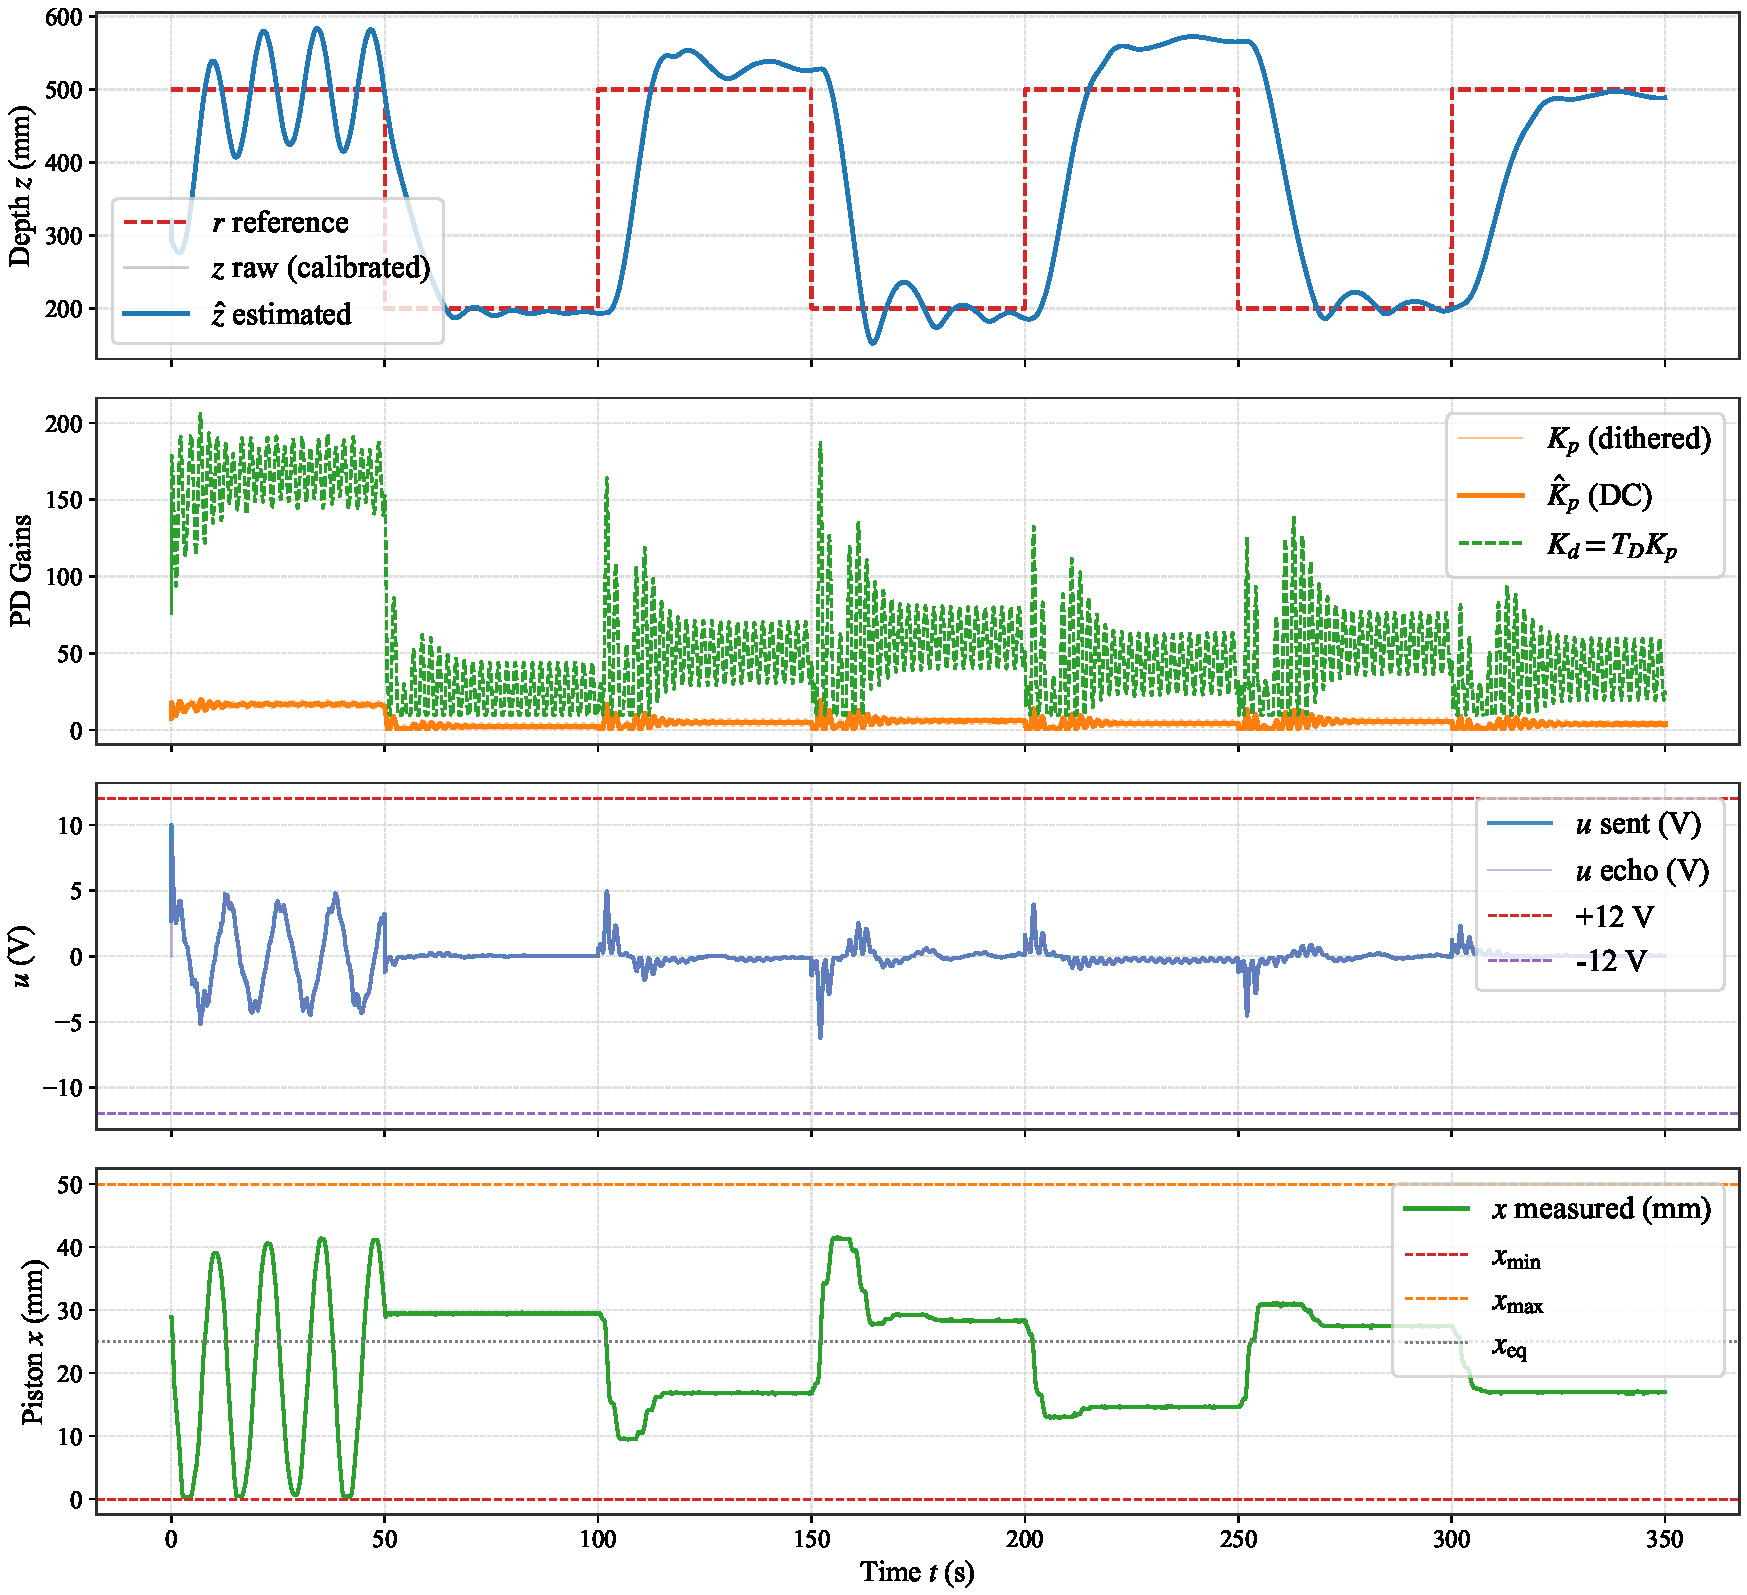
\includegraphics[width=0.65\textwidth]{Fig/ch3_esc_experiment.pdf}
    \caption{ESC experiment with online gain adaptation.}
    \label{fig:ch3_esc_experiment}
\end{figure}

These results show the tradeoff between MPC and ESC. MPC gives a structured way to enforce constraints when the model is reliable. ESC is less dependent on an exact model and can adapt to actuator dead zone and cable disturbance, but its performance depends strongly on objective-function design. For this BCD, the deadzone piston-position penalty is more directly tied to safe operation than a generic actuator-motion penalty.

\subsection{Simulator Results}

The simulator is used to compare PBVS and IBVS before implementing the real system. Figure~\ref{fig:ch3_simulator_responses} shows that both approaches can converge the visual-servoing error in simulation. The gains are not directly interchangeable because $\psi_e$ has a different physical meaning in each case. In PBVS, the error is formed from world-frame geometry. In IBVS, the error is formed from image-space features.

\begin{figure}[t]
    \centering
    \begin{minipage}{0.65\textwidth}
        \centering
        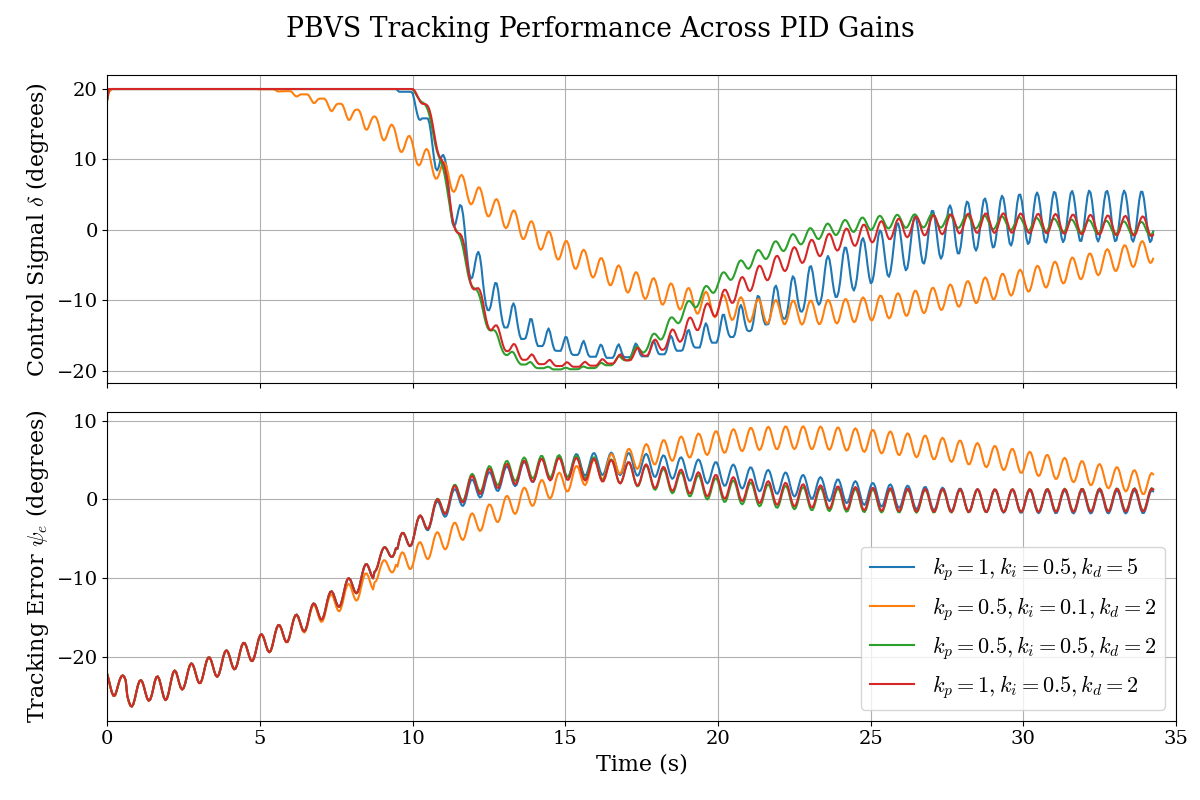
\includegraphics[width=\textwidth]{Fig/ch3_pbvs_simulation.png}
    \end{minipage}

    \begin{minipage}{0.65\textwidth}
        \centering
        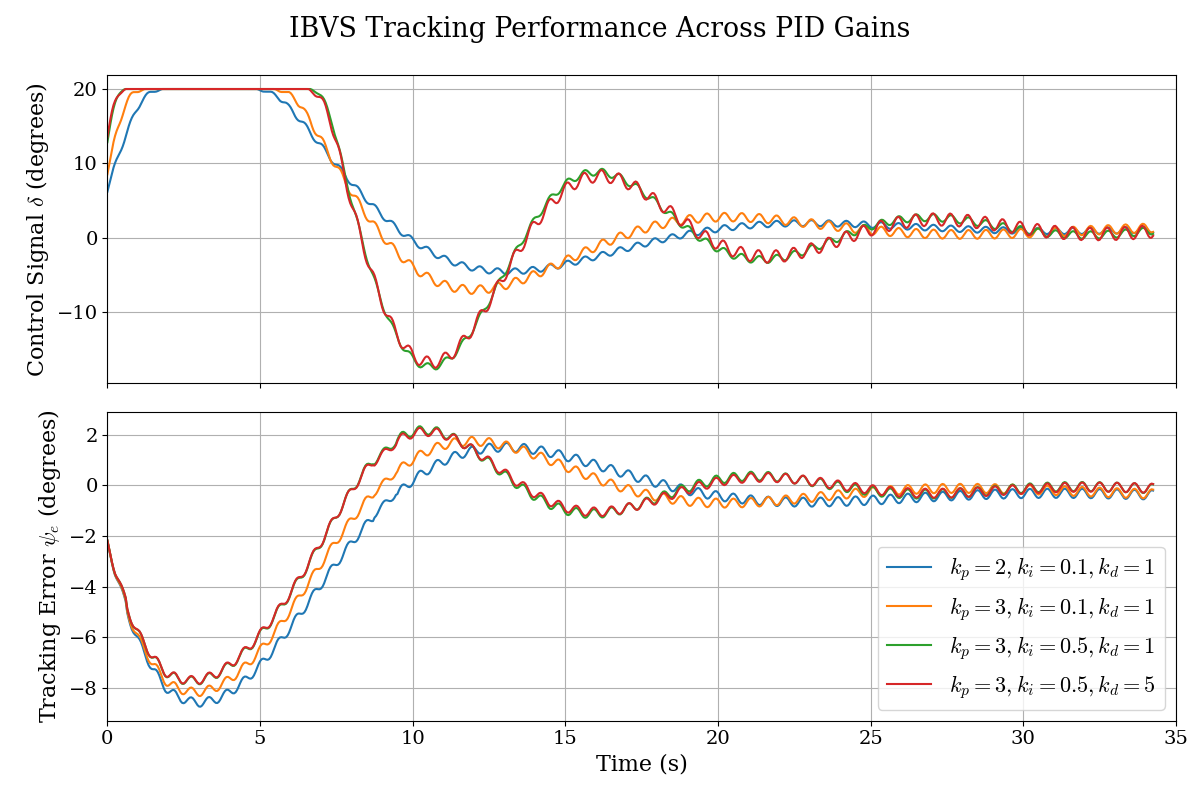
\includegraphics[width=\textwidth]{Fig/ch3_ibvs_simulation.png}
    \end{minipage}
    \caption{PBVS and IBVS simulator responses for pipeline tracking.}
    \label{fig:ch3_simulator_responses}
\end{figure}

The simulator supports controller tuning because it captures the underactuated planar dynamics and the oscillatory behavior introduced by tail propulsion. However, the physical experiment remains necessary because image noise, communication dropouts, lighting, water motion, and mechanical vibration are difficult to reproduce exactly. For AquaNavigator, the simulator is therefore used as a controller-development tool rather than as a substitute for pool validation.

\subsection{Pipeline Tracking Results}

The pipeline-tracking pool experiment evaluates whether the robotic fish can reduce the image-space heading error $\psi_e$ and move toward the detected pipeline. The experiment begins with the robot away from the pipeline, producing an initial $\psi_e$ of approximately $25^\circ$. As the controller redirects the tail-bias angle, $\psi_e$ converges toward zero and the robot continues along the pipeline. The control input reaches the $\pm 20^\circ$ saturation limit during parts of the transient.

The top-view sequence in Fig.~\ref{fig:ch3_pipeline_top_view} shows the pipeline-tracking experiment spatially. The fish moves toward the pipeline, aligns with it, and then continues along it with a steady heading.

\begin{figure}[t]
    \centering
    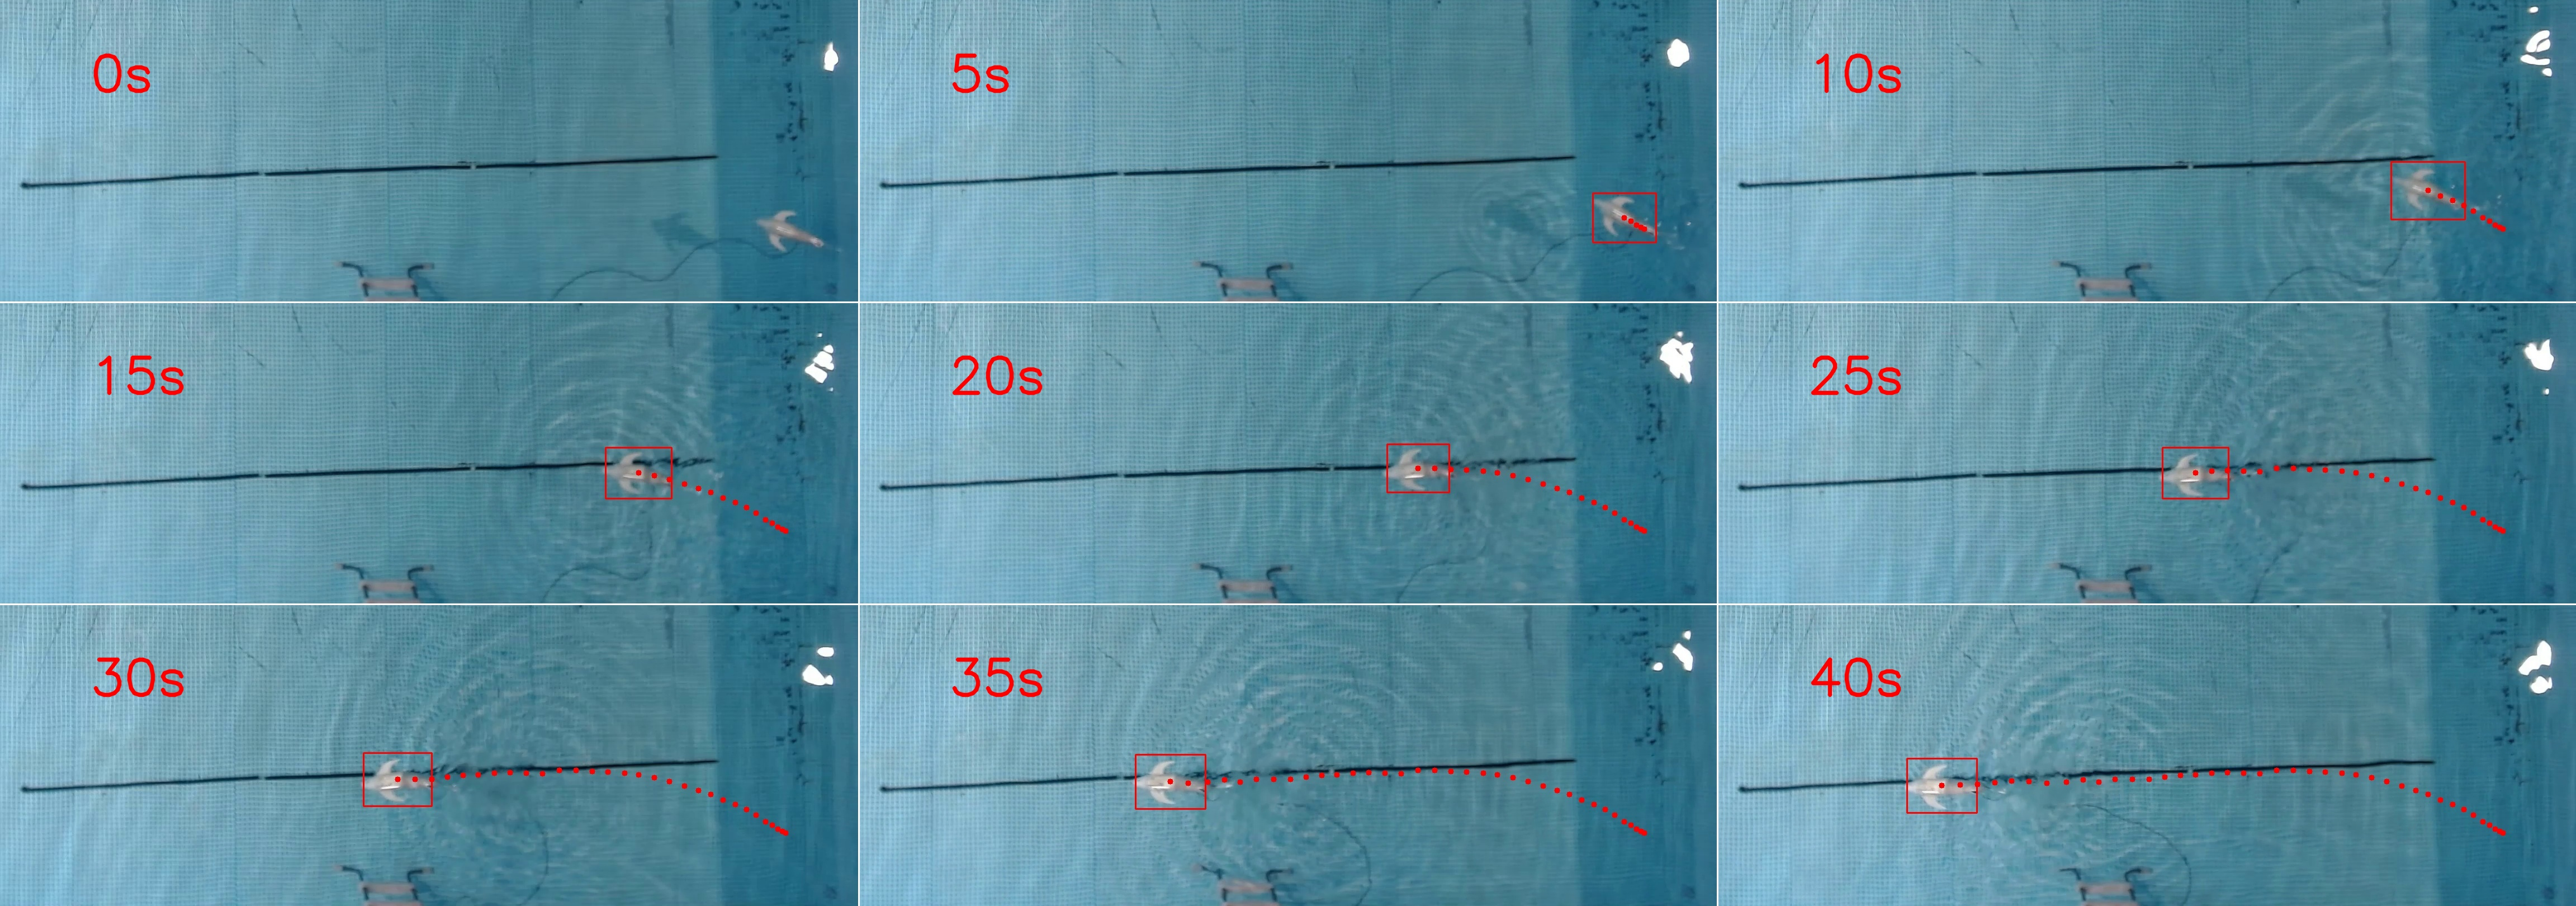
\includegraphics[width=0.94\textwidth]{Fig/ch3_pipeline_top_view.jpg}
    \caption{Top-view sequence of pipeline tracking experiment.}
    \label{fig:ch3_pipeline_top_view}
\end{figure}

\begin{table}[t]
    \centering
    \caption{Pipeline tracking pool experiment result summary.}
    \label{tab:ch3_pipeline_results}
    \begin{tabular}{lllll}
        \hline
        Test & Span (s) & Start $\psi_e$ (deg) & Start $y$ (pixels) & $t_s$ (s) \\
        \hline
        1 & 11 & 28 & -3 & 11 \\
        2 & 65 & 25 & 180 & 20 \\
        3 & 45 & 22 & 175 & 9 \\
        4 & 28 & 45 & -220 & 28 \\
        5 & 15 & -25 & 130 & 7 \\
        6 & 37 & -5 & 200 & 25 \\
        \hline
    \end{tabular}
\end{table}

Across the listed pool experiments, the robot converges to within $\psi_e=\pm 5^\circ$ of the pipeline. The settling time depends on the initial orientation and lateral offset. The result demonstrates pipeline following in a controlled indoor pool, not open-water industrial inspection. The visual signal is not perfectly smooth because the tail mechanism introduces body and camera oscillation. This is a real limitation of camera-guided robotic-fish control and must be considered when designing onboard perception and control.

\section{Conclusion}
The open-loop BCD validation gave an actuator-position RMSE of $1.96$~mm and a depth-response RMSE of $23.07$~mm, showing that the identified actuator dynamics were captured more tightly than the coupled depth response. The remaining depth error is consistent with unmodeled drag variation, tank-wall effects, and small neutral-buoyancy offsets in the laboratory setup. First an MPC controller was developed that used the model to enforce piston constraints and produced acceptable depth regulation while respecting actuator limits, but its performance depended on model fidelity. The ESC-tuned PD controller addressed this limitation by adapting gains online from measured performance while respecting voltage and stroke limits.

For the robotic fish, image-based visual servoing was used to track a pipeline-like feature by commanding the tail-bias angle, with the simulator supporting PBVS and IBVS comparison and gain tuning before pool experiments. The results show that the BCD and AquaNavigator can be controlled in constrained laboratory and pool settings, but they also show the limitations that motivate the next chapter. Pipeline tracking is a first inspection behavior, and depth regulation is a prerequisite for three-dimensional operation.

\chapter{Safety, Inspection, and Monitoring of Underwater Infrastructure}
% TODO: Add chapter introduction, pipeline tracking, CO2 monitoring,
% oil-spill sensing, results/discussion, and chapter conclusion.

\chapter{Cooperative Inspection: Relative Localization Framework}
% TODO: Add chapter introduction, relative-localization framework,
% validation results/discussion, and chapter conclusion.

\chapter{Conclusions and Future Work}
% TODO: Add final conclusions and future-work directions.

\backmatter

\addcontentsline{toc}{chapter}{REFERENCES} \nocite{*}
\bibliographystyle{plain}
\bibliography{references}

\appendix

\chapter{Appendix Title}
Appendices continue the main Arabic page numbering sequence.

\end{document}
